\documentclass[final]{hcmuitthesis}
% Config reference source file
\addbibresource{references/references.bib}


% Define metadata
% =========== Thay đổi thông tin tại phần này ===========
\upperuniname{ĐẠI HỌC QUỐC GIA THÀNH PHỐ HỒ CHÍ MINH}
\uniname{TRƯỜNG ĐẠI HỌC CÔNG NGHỆ THÔNG TIN}
\deptname{KHOA KHOA HỌC MÁY TÍNH}
\stumajor{THẠC SĨ NGÀNH KHOA HỌC MÁY TÍNH}
\title{GIẢI PHÁP KẾT HỢP ONTOLOGY VÀ MÔ HÌNH NGÔN NGỮ LỚN ĐỂ THIẾT KẾ HỆ THỐNG TƯ VẤN KIẾN THỨC VỀ QUY ĐỊNH ĐÀO TẠO SAU ĐẠI HỌC}
\titleen{INTEGRATING ONTOLOGY AND LARGE LANGUAGE MODELS TO DESIGN AN ADVISORY SYSTEM FOR POSTGRADUATE EDUCATION REGULATIONS}
\supervisor{GIẢNG VIÊN HƯỚNG DẪN}
\supervisorname{PGS. TS. NGUYỄN ĐÌNH HIỂN \\ TS. NGÔ QUỐC HƯNG}
\stuname{LÊ HỒNG HIỂN}
\stunamewithid{LÊ HỒNG HIỂN - 210101006}
\reporttype{LUẬN VĂN THẠC SĨ}
\instruction{GIẢNG VIÊN HƯỚNG DẪN}
\reportplace{TP. HỒ CHÍ MINH, NĂM }

% =========== Hết phần thay đổi thông tin ===========

\newglossaryentry{kg}{
    name={KG},
    description={Knowledge Graph}
}

\newglossaryentry{llm}{
    name={LLM},
    description={Large Language Model}
}

\newglossaryentry{rag}{
    name={RAG},
    description={Retrieval-Augmented Generation}
}

\newglossaryentry{ppr}{
    name={PPR},
    description={Personalized PageRank}
}

\newglossaryentry{rrf}{
    name={RRF},
    description={Reciprocal Rank Fusion}
}

\newglossaryentry{owl}{
    name={OWL},
    description={Web Ontology Language}
}

\makeglossaries
% Begin thesis
\begin{document}

\coverpage%
\secondcoverpage%

% Begin above main thesis
\frontmatter
\chapter*{\centering\Large{Thông tin hội đồng chấm luận văn thạc sĩ}}
\addcontentsline{toc}{chapter}{Thông tin hội đồng chấm luận văn thạc sĩ}
Hội đồng chấm luận văn thạc sĩ, thành lập theo Quyết định số.../QĐ-ĐHCNTT ngày ... tháng ... năm 2026 của Hiệu trưởng Trường Đại học Công nghệ Thông tin.
\begin{center}
    \begin{tabular}{ p{.5\textwidth} p{.3\textwidth}}
        1. ...  & Chủ tịch \\
        2. ...  & Phản biện 1 \\
        3. ...  & Phản biện 2 \\
        4. ...  & Ủy viên \\
        5. ...  & Thư ký \\
    \end{tabular}
\end{center}

\chapter*{\centering\Large{Lời cam đoan}}
\addcontentsline{toc}{chapter}{Lời cam đoan}

Tôi xin cam đoan đây là công trình nghiên cứu của riêng tôi, được thực hiện dưới sự hướng dẫn khoa học của PGS. TS. Nguyễn Đình Hiển và TS. Ngô Quốc Hưng. Các số liệu, kết quả nêu trong luận văn là trung thực và chưa từng được ai công bố trong bất kỳ công trình nào khác.

Tôi xin chịu trách nhiệm về nghiên cứu của mình.

\begin{flushright}
\textit{Thành phố Hồ Chí Minh, ngày 04 tháng 05 năm 2026} \\
\textit{Người thực hiện} \\[1cm]
\textit{Lê Hồng Hiển}
\end{flushright}

\chapter*{\centering\Large{Lời cảm ơn}}
\addcontentsline{toc}{chapter}{Lời cảm ơn}

Xin chân thành cảm ơn quý thầy cô trong trường Đại học Công Nghệ Thông Tin, ĐHQG-HCM đã tận tình dạy bảo cho em nhiều kiến thức bổ ích trong suốt thời gian học tập tại trường, cũng như tạo điều kiện cho em thực hiện đề tài này. Kính chúc quý thầy cô luôn dồi dào sức khoẻ và thành công trong cuộc sống.

Đặc biệt, em xin bày tỏ lòng biết ơn chân thành đến PGS. TS. Nguyễn Đình Hiển, người thầy đã tận tâm, nhiệt tình hướng dẫn và chỉ bảo cho em trong suốt quá trình thực hiện đề tài. Em cũng xin gửi lời cảm ơn đến TS. Ngô Quốc Hưng (University College Dublin), người đồng hướng dẫn đã hỗ trợ về mặt học thuật quốc tế và đóng góp nhiều góp ý về phương pháp nghiên cứu.

Tôi cũng xin gửi lời cảm ơn đến ThS. Đặng Việt Dũng đã hỗ trợ và giúp đỡ tôi trong quá trình nghiên cứu.

Tôi cũng không quên gửi lời cảm ơn đến tác giả của các báo cáo nghiên cứu khoa học mà tôi đã tham khảo và tìm hiểu cho đề tài.

Luận văn đã hoàn thành với một số kết quả nhất định tuy nhiên vẫn không tránh khỏi thiếu sót. Kính mong sự cảm thông và đóng góp ý kiến từ quý thầy cô và các bạn.

Một lần nữa tôi xin chân thành cảm ơn!

\begin{flushright}
\textit{Thành phố Hồ Chí Minh, ngày 04 tháng 05 năm 2026} \\
\textit{Người thực hiện} \\[1cm]
\textit{Lê Hồng Hiển}
\end{flushright}

\tableofcontents
\clearpage
\listoffigures
\clearpage
\listoftables
\clearpage
\chapter*{\centering\Large{Danh mục từ tạm dịch}}
\addcontentsline{toc}{chapter}{Danh mục từ tạm dịch}
\begin{tabular}{| p{.4\textwidth} |p{.4\textwidth} |}
\hline
        \textbf{Tiếng Anh} & \textbf{Tiếng Việt} \\
        \hline
        Knowledge Graph & Đồ thị tri thức \\
        \hline
        Ontology & Bản thể học \\
        \hline
        Retrieval-Augmented Generation & Retrieval-Augmented Generation (RAG) \\
        \hline
        Large Language Model & Mô hình ngôn ngữ lớn \\
        \hline
        Tree Traversal & Duyệt cây \\
        \hline
        Semantic Retrieval & Truy xuất ngữ nghĩa \\
        \hline
        Reciprocal Rank Fusion & Reciprocal Rank Fusion (RRF) \\
        \hline
        Personalized PageRank & PageRank cá nhân hóa \\
        \hline
        Document Forest & Rừng cây tài liệu \\
        \hline
        Cross-reference & Tham chiếu chéo \\
        \hline
        Embedding & Biểu diễn nhúng \\
        \hline
        Hallucination & Ảo giác \\
        \hline
        Query Intent & Ý định truy vấn \\
        \hline
        Hit Rate & Tỷ lệ trúng \\
        \hline
        Mean Reciprocal Rank & Hạng nghịch đảo trung bình \\
        \hline
        Summary Tree & Cây tóm tắt \\
        \hline
        Document Tree & Cây tài liệu \\
        \hline
        Multi-hop Reasoning & Suy luận đa bước \\
        \hline
        Knowledge Graph Expansion & Mở rộng đồ thị tri thức \\
        \hline
\end{tabular}

\clearpage
\mainthesis

% Main chapter in thesis
% ============================================================
%  Chương 1: Tổng quan
% ============================================================
\chapter{Tổng quan}
\label{chap:chapter1}

Chương này trình bày tổng quan về đề tài nghiên cứu, bao gồm giới thiệu bối cảnh và động lực nghiên cứu, tổng quan các công trình liên quan, mục tiêu và phạm vi nghiên cứu, cũng như bố cục của luận văn.

% ============================================================
\section{Giới thiệu đề tài}
\label{sec:gioithieu}

% ------------------------------------------------------------
\subsection{Bối cảnh và động lực nghiên cứu}
\label{subsec:boicanh}

Tại các trường đại học ở Việt Nam, nhiều phòng ban chức năng đã được thành lập để hỗ trợ sinh viên trong học tập, rèn luyện và giải quyết các thủ tục hành chính. Tuy nhiên, do thông tin bị phân tán giữa nhiều phòng ban và các quy định thường khó hiểu, sinh viên gặp nhiều trở ngại trong việc tra cứu, tiếp cận và nắm bắt đầy đủ các quy định đào tạo, nhất là đối với những quy chế mới hoặc có tính chất phức tạp. Sinh viên thường phải liên hệ với nhiều nơi khác nhau cho từng vấn đề, dẫn đến mất thời gian, chờ đợi kéo dài và đôi khi không nhận được thông tin chính xác, kịp thời.

Ngoài ra, các nhu cầu tư vấn về học tập, nghiên cứu khoa học, lựa chọn ngành nghề, điều kiện tốt nghiệp cũng ngày càng đa dạng, trong khi nguồn lực cán bộ tư vấn còn hạn chế. Việc giải thích các quy định đào tạo phức tạp thường đòi hỏi sự tương tác trực tiếp, gây áp lực lớn cho đội ngũ cán bộ và không đáp ứng được nhu cầu hỗ trợ 24/7. Do đó, việc xây dựng một hệ thống tư vấn tự động, thông minh sẽ giúp giảm tải cho cán bộ, tiết kiệm chi phí vận hành, đồng thời nâng cao trải nghiệm và sự hài lòng của sinh viên.

% ------------------------------------------------------------
\subsection{Hiện trạng các hệ thống chatbot giáo dục tại Việt Nam}
\label{subsec:hientrang}

Gần đây, nhiều trường đại học tại Việt Nam đã tiên phong ứng dụng trí tuệ nhân tạo vào các hệ thống hỗ trợ sinh viên:
\begin{itemize}
    \item \textbf{Chatbot UEB} (Đại học Kinh tế Quốc dân): triển khai dựa trên nền tảng ChatGPT, giúp sinh viên tra cứu thông tin và giải đáp thắc mắc mọi lúc, mọi nơi.
    \item \textbf{UEH AI Chatbot} (Đại học Kinh tế TP.HCM): hỗ trợ tư vấn tuyển sinh, hướng nghiệp cho phụ huynh và học sinh.
    \item \textbf{HUNRE AI Chatbot} (Đại học Tài nguyên và Môi trường Hà Nội): góp phần nâng cao chất lượng phục vụ sinh viên và tối ưu hóa quy trình quản lý đào tạo.
\end{itemize}

Các ứng dụng chatbot này chủ yếu dựa trên mô hình ngôn ngữ lớn (LLM), đã được triển khai rộng rãi và bước đầu mang lại nhiều tiện ích cho sinh viên. Tuy nhiên, hiện vẫn còn thiếu các nghiên cứu đánh giá định lượng về mức độ chính xác và hiệu quả thực sự của các hệ thống này. Bên cạnh đó, các LLM hiện nay vẫn gặp nhiều hạn chế trong việc xử lý các câu hỏi phức tạp đòi hỏi suy luận logic sâu. Đặc biệt, hiện tượng \textit{``ảo giác''} (hallucination), tức khi mô hình tạo ra câu trả lời không chính xác hoặc không sát với thực tế, vẫn là một rào cản lớn, có thể dẫn đến việc cung cấp thông tin sai lệch với hậu quả nghiêm trọng đối với sinh viên.

% ------------------------------------------------------------
\subsection{Thách thức trong truy xuất thông tin văn bản quy phạm}
\label{subsec:thachchuc}

Các văn bản quy chế đào tạo tại Việt Nam có cấu trúc phân cấp phức tạp: một quy chế tổ chức nội dung theo các cấp Chương, Điều, Khoản và Điểm, mỗi cấp mang phạm vi quy định riêng biệt. Ngoài ra, các văn bản còn chứa nhiều tham chiếu chéo (cross-reference): để trả lời câu hỏi \textit{``Học viên cao học cần đáp ứng điều kiện gì để được bảo vệ luận văn?''} cần kết nối Điều~24 (điều kiện bảo vệ) trong QĐ~270 của UIT với Điều~25 (yêu cầu ngoại ngữ) trong QĐ~1393 của ĐHQG-HCM, vốn là hai văn bản khác nhau ở hai tầng quản lý.

Tiếng Việt còn tạo thêm thách thức qua sự đa nghĩa thanh điệu, các viết tắt chuyên ngành (GVHD, ThS, NCS, ĐHQG) và hệ thống phân cấp văn bản quy phạm đa tầng (Bộ GD\&ĐT, ĐHQG-HCM, trường thành viên). Các phương pháp truy xuất thông tin truyền thống dựa trên vector similarity~\cite{reimers2019sbert} hiệu quả trong nhiều lĩnh vực~\cite{fan2024ragsurvey} nhưng không đủ cho văn bản quy phạm có cấu trúc: embedding mờ đi ý nghĩa chính xác của thuật ngữ chuyên ngành (\textit{semantic gap}), truy xuất phẳng bỏ qua cấu trúc phân cấp tài liệu, và tìm kiếm dày đặc không thể kết nối các tham chiếu chéo giữa các quy chế. Các thách thức tương tự cũng xuất hiện trong lĩnh vực pháp luật Việt Nam, nơi hệ thống được mở rộng đánh giá (Chương~\ref{chap:chapter4}).

% ============================================================
\section{Các nghiên cứu liên quan}
\label{sec:lienquan}

% ------------------------------------------------------------
\subsection{Từ truy xuất từ vựng đến truy xuất neural}
\label{subsec:truyxuat_tuvung}

Truy xuất thông tin pháp lý ban đầu dựa vào đối sánh từ vựng: BM25~\cite{robertson2009bm25} và TF-IDF~\cite{manning2008ir} xếp hạng tài liệu theo mức độ trùng khớp thuật ngữ, nhưng thất bại khi người dùng diễn đạt lại các khái niệm pháp lý bằng ngôn ngữ tự nhiên. Truy xuất dày đặc (dense retrieval) chuyển sang các biểu diễn học được với Sentence-BERT~\cite{reimers2019sbert} và DPR~\cite{karpukhin2020dpr}; các công trình tiếp theo bổ sung cơ chế tự phản ánh~\cite{asai2024selfrag} và sinh tài liệu giả thuyết~\cite{gao2023hyde} (được tổng quan bởi Fan và cộng sự~\cite{fan2024ragsurvey}). Các mô hình chuyên biệt miền như LEGAL-BERT~\cite{chalkidis2020legalbert} nắm bắt ngôn ngữ pháp lý nhưng vẫn hoạt động trên các đoạn văn bản phẳng.

Đối với tiếng Việt, PhoBERT~\cite{nguyen2020phobert} và VnCoreNLP~\cite{vu2018vncore} cung cấp các mô hình nền tảng, và Ngo cùng cộng sự~\cite{ngo2021aimelaw} đã kết hợp BM25 với BERT~\cite{devlin2019bert} cho cuộc thi ALQAC~2021. Một hạn chế chung xuyên suốt các phương pháp này: việc coi tài liệu như tập hợp phẳng đã loại bỏ cấu trúc phân cấp quan trọng cho văn bản pháp lý.

% ------------------------------------------------------------
\subsection{Truy xuất tăng cường tri thức}
\label{subsec:truyxuat_trithuc}

Để phục hồi thông tin có cấu trúc và quan hệ, các nhà nghiên cứu đã chuyển sang các mô hình biểu diễn tri thức. Legal-Onto~\cite{nguyen2022legalonto} kết hợp mô hình Rela~\cite{do2018rela} với đồ thị khái niệm cho Luật Đất đai Việt Nam nhưng dựa vào luật thủ công, không có khả năng mở rộng. GraphRAG~\cite{edge2024graphrag} phân vùng đồ thị thực thể thành các cộng đồng với tóm tắt LLM, và LightRAG~\cite{guo2025lightrag} kết hợp tìm kiếm vector với duyệt đồ thị. Cả hai cho phép suy luận đa bước nhưng coi tài liệu như tập hợp thực thể mà không bảo toàn cấu trúc phân cấp; trong thử nghiệm của chúng tôi, chất lượng trích xuất thực thể của LightRAG khá thấp (74\% thực thể chỉ xuất hiện một lần).

RAG~\cite{lewis2020rag} nền tảng hóa việc sinh văn bản dựa trên bằng chứng truy xuất nhưng vẫn bị giới hạn bởi chất lượng truy xuất. Các khảo sát~\cite{zhong2020nlplaw,lai2024llmlaw} xác nhận rằng việc kết nối tri thức pháp lý với truy xuất có khả năng mở rộng vẫn là một vấn đề mở.

% ------------------------------------------------------------
\subsection{Truy xuất phân cấp nhận biết cấu trúc}
\label{subsec:truyxuat_phancap}

RAPTOR~\cite{sarthi2024raptor} xây dựng Summary Tree qua phân cụm đệ quy và tóm tắt LLM, nắm bắt chủ đề đa mức chi tiết; tuy nhiên, nó loại bỏ cấu trúc phân cấp gốc của tài liệu và chỉ dựa vào truy xuất embedding tại thời điểm truy vấn, chỉ đạt 41,0\% tỷ lệ Hit@10 trên bộ đánh giá pháp lý có cấu trúc của chúng tôi.

PageIndex~\cite{zhang2025pageindex} duyệt qua cây theo hướng dẫn bởi LLM để tìm kiếm tài liệu đã phân cấp, đạt độ chính xác cao khi mô hình chọn đúng nhánh nhưng bỏ sót nội dung ngoài đường duyệt. Đặc biệt, cả hai hệ thống đều không tích hợp Knowledge Graph cho suy luận liên tài liệu; các truy vấn đa bước xuyên các luật hoặc nghị định khác nhau chưa được giải quyết.

% ------------------------------------------------------------
\subsection{Định vị nghiên cứu}
\label{subsec:dinhvi}

Chưa có hệ thống nào kết hợp tri thức ontology, truy xuất dựa trên đồ thị và duyệt cây cấu trúc cho văn bản pháp lý Việt Nam. Hệ thống được đề xuất trong luận văn này tích hợp cả ba khả năng thông qua kiến trúc ba tầng với suy luận nhận biết ý định và tổng hợp, xếp hạng. Bảng~\ref{tab:comparison} tóm tắt so sánh các phương pháp liên quan.

\begin{table}[htbp]
    \centering
    \caption{So sánh các hệ thống liên quan}
    \label{tab:comparison}
    \resizebox{\textwidth}{!}{\begin{tabular}{lcccc}
        \toprule
        \textbf{Hệ thống} & \textbf{Cấu trúc} & \textbf{KG} & \textbf{Ngữ nghĩa} & \textbf{Đa tài liệu} \\
        \midrule
        BM25/TF-IDF                  & --             & --  & --  & \checkmark \\
        NaiveRAG                     & --             & --  & \checkmark & \checkmark \\
        LightRAG~\cite{guo2025lightrag}  & --         & \checkmark & \checkmark & \checkmark \\
        RAPTOR~\cite{sarthi2024raptor}   & Summary Tree & --  & \checkmark & \checkmark \\
        PageIndex~\cite{zhang2025pageindex} & Document Tree & -- & -- & \checkmark \\
        Legal-Onto~\cite{nguyen2022legalonto} & --    & \checkmark & -- & -- \\
        \textbf{3-Tier (ours)}       & Document Tree  & \checkmark & \checkmark & \checkmark \\
        \bottomrule
    \end{tabular}}
\end{table}

% ============================================================
\section{Mục tiêu và phạm vi nghiên cứu}
\label{sec:muctieu}

% ------------------------------------------------------------
\subsection{Mục tiêu nghiên cứu}
\label{subsec:muctieu_nc}

Luận văn này nghiên cứu và giải quyết các vấn đề sau:
\begin{enumerate}
    \item \textbf{Xây dựng Knowledge Graph và Ontology cho văn bản quy phạm:} Xây dựng pipeline trích xuất tri thức bán tự động sử dụng LLM để trích xuất thực thể và quan hệ từ văn bản quy phạm, kết hợp tinh chỉnh bởi chuyên gia (expert-in-the-loop) để tạo KG. Từ KG đã xây dựng, suy luận (infer) ontology chuyên biệt theo chuẩn OWL, xác định hệ thống phân cấp các loại thực thể (chủ thể, điều kiện, thời hạn, mức phạt, \ldots) và quan hệ (references, requires, depends\_on, \ldots), phục vụ cho cơ chế Concept Matching trong truy xuất ngữ nghĩa.

    \item \textbf{Đề xuất kiến trúc truy xuất 3-Tier KG-RAG:} Thiết kế kiến trúc truy xuất ba tầng kết hợp duyệt cây cấu trúc hướng dẫn bởi LLM (Tầng~1), truy xuất ngữ nghĩa hai cấp dựa trên KG và embedding (Tầng~2), và hợp nhất Reciprocal Rank Fusion với mở rộng Knowledge Graph (Tầng~3). Kiến trúc này tận dụng đồng thời cấu trúc phân cấp của văn bản quy phạm, quan hệ ngữ nghĩa trong đồ thị tri thức và tín hiệu tương đồng vector để truy xuất chính xác các điều khoản liên quan.

    \item \textbf{Xây dựng bộ đánh giá và so sánh định lượng:} Thiết kế các bộ benchmark tiếng Việt gồm các câu hỏi phức tạp yêu cầu suy luận đa bước, tham chiếu chéo giữa các văn bản. Đánh giá hệ thống bằng các chỉ số Hit@k và MRR, so sánh với các phương pháp tiên tiến (PageIndex, RAPTOR, LightRAG), và phân tích ablation để đo lường đóng góp của từng thành phần.
\end{enumerate}

% ------------------------------------------------------------
\subsection{Đối tượng}
\label{subsec:doituong}

Đề tài này nghiên cứu việc tổ chức và truy xuất thông tin từ các văn bản quy phạm có cấu trúc phân cấp để xây dựng một hệ thống hỏi đáp tự động dựa trên đồ thị tri thức và mô hình ngôn ngữ lớn. Hệ thống hướng đến đối tượng là học viên cao học, sinh viên sau đại học tại UIT và các trường thuộc ĐHQG-HCM có nhu cầu tra cứu các quy định đào tạo, cũng như cán bộ phòng đào tạo cần hỗ trợ giải đáp thắc mắc cho học viên. Hệ thống cũng có thể mở rộng ra cho người dùng có nhu cầu muốn tra cứu thông tin pháp luật.

% ------------------------------------------------------------
\subsection{Phạm vi nghiên cứu}
\label{subsec:phamvi}

Hệ thống được kiểm thử trên 5 bộ quy chế, quy định đào tạo thạc sĩ:
\begin{enumerate}
    \item Quy chế đào tạo trình độ thạc sĩ của UIT số 270/QĐ-ĐHCNTT ngày 25/04/2022.
    \item Quy chế đào tạo trình độ thạc sĩ cho khóa 2021 số 160/QĐ-ĐHQG ngày 24/03/2017 của ĐHQG-HCM.
    \item Quy chế đào tạo trình độ thạc sĩ cho khóa từ năm 2022 số 1393/QĐ-ĐHQG ngày 03/11/2021 của ĐHQG-HCM.
    \item Quy chế sửa đổi bổ sung số 218/QĐ-ĐHQG ngày 15/03/2024 của ĐHQG-HCM.
    \item Quy định về liêm chính học thuật số 851/QĐ-ĐHCNTT ngày 14/08/2024 của UIT.
\end{enumerate}

Ngoài ra, hệ thống còn được đánh giá trên bộ dữ liệu pháp luật Việt Nam gồm 12 văn bản thuộc lĩnh vực luật doanh nghiệp và luật giao thông để chứng minh tính tổng quát của phương pháp.

% ============================================================
\section{Bố cục luận văn}
\label{sec:bocuc}

Phần còn lại của luận văn được tổ chức như sau:
\begin{itemize}
    \item \textbf{Chương~2}: Thu thập kiến thức về quy định đào tạo: trình bày tổng quan hệ thống quy chế đào tạo thạc sĩ, quy trình thu thập và tổ chức kiến thức từ văn bản quy phạm, cũng như xây dựng bộ câu hỏi kiểm thử.
    \item \textbf{Chương~3}: Thiết kế giải thuật: trình bày chi tiết kiến trúc 3-Tier KG-RAG bao gồm phân tích truy vấn, duyệt cây cấu trúc, truy xuất ngữ nghĩa hai cấp và hợp nhất RRF với mở rộng Knowledge Graph.
    \item \textbf{Chương~4}: Thiết kế hệ thống và thử nghiệm: trình bày yêu cầu hệ thống, kiến trúc triển khai, và kết quả thử nghiệm trên hai nghiên cứu trường hợp (case study) cùng phân tích ablation.
    \item \textbf{Chương~5}: Kết luận và hướng phát triển: tổng kết các kết quả đạt được, thảo luận hạn chế và đề xuất hướng phát triển tương lai.
\end{itemize}

% ============================================================
%  Chương 2: Thu thập kiến thức về quy định đào tạo
% ============================================================
\chapter{Thu thập kiến thức về quy định đào tạo}
\label{chap:chapter2}

Chương này trình bày tổng quan về hệ thống quy chế đào tạo thạc sĩ tại UIT và ĐHQG-HCM, quy trình thu thập và tổ chức kiến thức từ các văn bản quy phạm, cũng như việc xây dựng bộ câu hỏi kiểm thử phục vụ đánh giá hệ thống. Nội dung chương này tuân theo phương pháp thu thập kiến thức theo miền (domain knowledge acquisition) cho hệ thống truy xuất thông tin.

% ============================================================
\section{Giới thiệu về hệ thống quy chế đào tạo thạc sĩ}
\label{sec:gioithieu_quyche}

% ------------------------------------------------------------
\subsection{Tổng quan hệ thống quy chế đào tạo sau đại học tại Việt Nam}
\label{subsec:tongquan_hethong}

Hệ thống giáo dục sau đại học tại Việt Nam được quản lý bởi nhiều tầng văn bản quy phạm pháp luật, từ cấp quốc gia đến cấp trường. Tại cấp quốc gia, Luật Giáo dục và Luật Giáo dục Đại học đặt ra khung pháp lý chung. Bộ Giáo dục và Đào tạo ban hành các quy chế đào tạo trình độ thạc sĩ, tiến sĩ áp dụng trên toàn quốc. Tại cấp cơ sở, các đại học quốc gia và trường đại học ban hành quy chế riêng phù hợp với đặc thù đào tạo.

Đối với UIT, một trường thành viên của ĐHQG-HCM, hệ thống quy chế đào tạo thạc sĩ bao gồm hai tầng chính:
\begin{itemize}
    \item \textbf{Tầng ĐHQG-HCM}: Các quy chế khung do ĐHQG-HCM ban hành, áp dụng cho tất cả các trường thành viên (QĐ~160, QĐ~1393, QĐ~218).
    \item \textbf{Tầng trường}: Các quy chế, quy định cụ thể hóa do UIT ban hành (QĐ~270, QĐ~851), bổ sung và chi tiết hóa các quy định của ĐHQG-HCM.
\end{itemize}

% ------------------------------------------------------------
\subsection{Cấu trúc văn bản quy phạm}
\label{subsec:cautruc_vanban}

Các văn bản quy chế đào tạo tuân theo cấu trúc phân cấp chuẩn của văn bản quy phạm pháp luật Việt Nam. Từ cấp cao nhất đến cấp thấp nhất, cấu trúc được tổ chức như sau:

\[
\text{Văn bản} \rightarrow \text{Chương} \rightarrow \text{Mục} \rightarrow \text{Điều} \rightarrow \text{Khoản} \rightarrow \text{Điểm}
\]

Mỗi cấp trong hệ thống phân cấp mang một phạm vi quy định riêng biệt. \textit{Văn bản} là đơn vị pháp lý cao nhất, xác định phạm vi và đối tượng áp dụng. \textit{Chương} nhóm các quy định theo chủ đề lớn. \textit{Mục} (nếu có) phân nhỏ chương theo nhóm điều liên quan. \textit{Điều} là đơn vị quy định cơ bản, mang nội dung pháp lý cụ thể. \textit{Khoản} cụ thể hóa từng khía cạnh của Điều. \textit{Điểm} liệt kê các trường hợp hoặc điều kiện chi tiết trong Khoản.

Ngoài cấu trúc phân cấp dọc, các văn bản còn tồn tại các tham chiếu chéo ngang giữa các điều khoản trong cùng một văn bản hoặc giữa các văn bản khác nhau. Ví dụ, để xác định điều kiện bảo vệ luận văn thạc sĩ, cần đọc Điều~24 trong QĐ~270 kết hợp với Điều~25 trong QĐ~1393, hai văn bản thuộc hai tầng quản lý khác nhau.

Hình~\ref{fig:document_tree} minh họa cấu trúc Document Tree của QĐ~270/QĐ-ĐHCNTT với sáu cấp phân cấp và các liên kết tham chiếu chéo giữa các điều.

\begin{figure}[htbp]
    \centering
    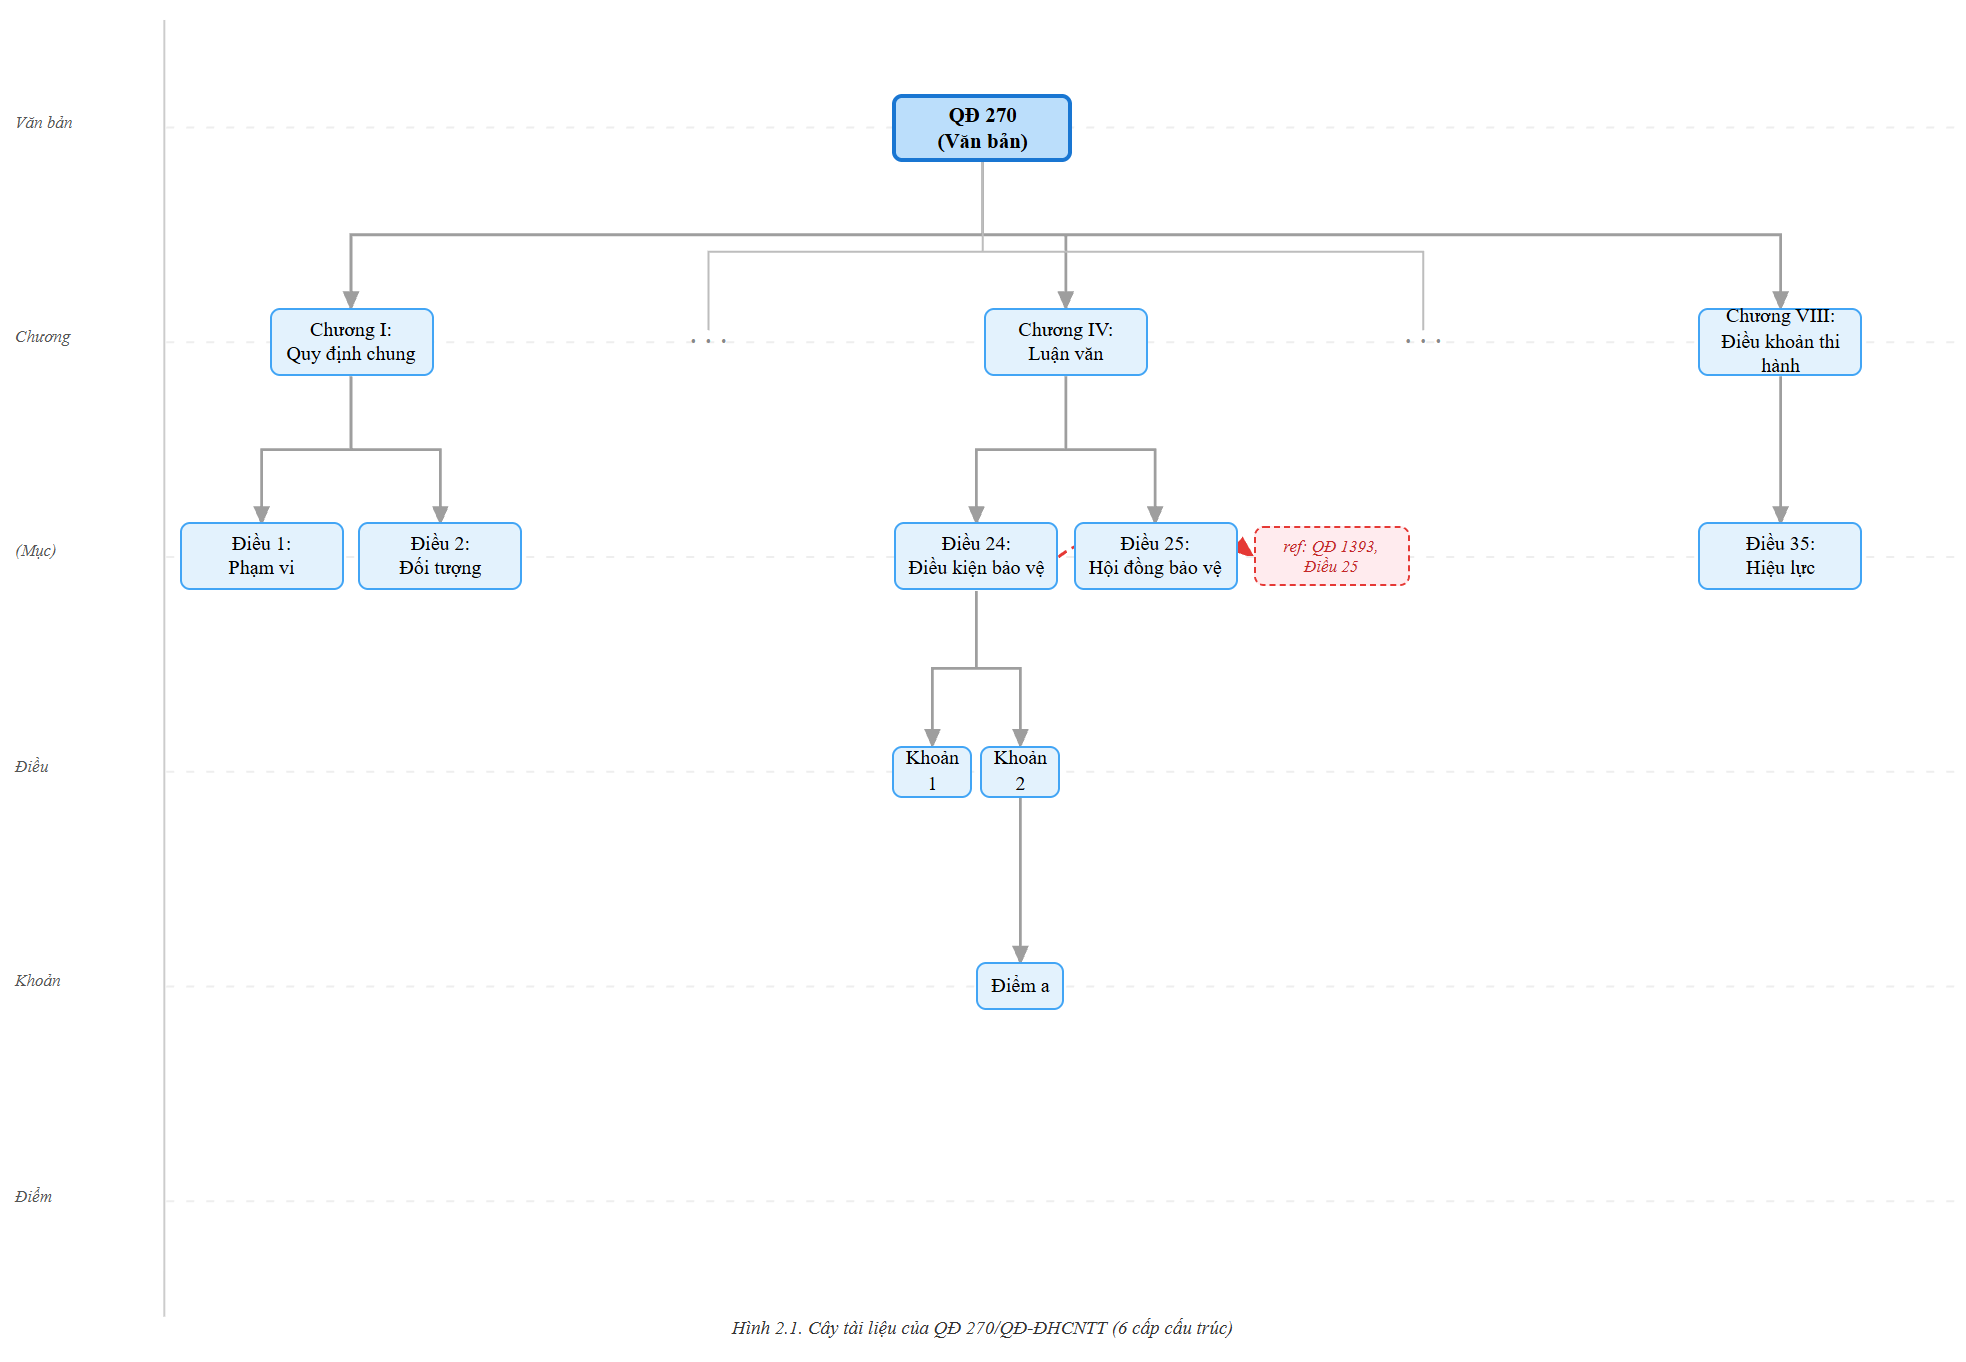
\includegraphics[width=0.95\textwidth]{graphics/figure2-1-document-tree.png}
    \caption{Cấu trúc Document Tree của QĐ~270/QĐ-ĐHCNTT (minh họa rút gọn). Mũi tên nét đứt thể hiện tham chiếu chéo giữa các điều.}
    \label{fig:document_tree}
\end{figure}

% ------------------------------------------------------------
\subsection{Các quy chế trong phạm vi nghiên cứu}
\label{subsec:cacquiche}

Bảng~\ref{tab:quyche_list} liệt kê năm văn bản quy chế đào tạo trong phạm vi nghiên cứu của luận văn.

\begin{table}[htbp]
    \centering
    \caption{Danh sách các quy chế đào tạo trong phạm vi nghiên cứu}
    \label{tab:quyche_list}
    \begin{tabular}{clccc}
        \toprule
        \textbf{STT} & \textbf{Tên quy chế} & \textbf{Số QĐ} & \textbf{Số chương} & \textbf{Số điều} \\
        \midrule
        1 & Quy chế ĐT trình độ ThS của UIT
          & 270/QĐ-ĐHCNTT & 8 & 35 \\
        2 & Quy chế ĐT trình độ ThS ĐHQG-HCM (khóa 2021)
          & 160/QĐ-ĐHQG & 7 & 28 \\
        3 & Quy chế ĐT trình độ ThS ĐHQG-HCM (khóa 2022+)
          & 1393/QĐ-ĐHQG & 8 & 32 \\
        4 & Quy chế sửa đổi bổ sung về GVHD
          & 218/QĐ-ĐHQG & 2 & 6 \\
        5 & Quy định liêm chính học thuật
          & 851/QĐ-ĐHCNTT & 3 & 8 \\
        \midrule
        \multicolumn{3}{r}{\textbf{Tổng cộng}} & \textbf{28} & \textbf{109} \\
        \bottomrule
    \end{tabular}
\end{table}

\textbf{QĐ~270/QĐ-ĐHCNTT} là quy chế đào tạo thạc sĩ chủ đạo của UIT, ban hành ngày 25/04/2022. Quy chế gồm 8~chương và 35~điều, bao phủ toàn bộ quy trình đào tạo thạc sĩ tại UIT từ tuyển sinh, tổ chức đào tạo, đến bảo vệ và cấp bằng. Đây là văn bản cụ thể hóa các quy định của ĐHQG-HCM, có tính đặc thù cao cho UIT.

\textbf{QĐ~160/QĐ-ĐHQG} là quy chế đào tạo thạc sĩ của ĐHQG-HCM áp dụng cho khóa tuyển sinh năm 2021 trở về trước, gồm 7~chương và 28~điều, quy định về tổ chức và quản lý đào tạo trình độ thạc sĩ trong toàn hệ thống ĐHQG-HCM.

\textbf{QĐ~1393/QĐ-ĐHQG} là quy chế thay thế QĐ~160 áp dụng từ khóa tuyển sinh năm 2022 trở đi, gồm 8~chương và 32~điều. Quy chế này có nhiều điểm mới về yêu cầu ngoại ngữ, điều kiện bảo vệ luận văn và hình thức đào tạo.

\textbf{QĐ~218/QĐ-ĐHQG} là quy chế sửa đổi bổ sung một số điều liên quan đến giảng viên hướng dẫn (GVHD), gồm 2~chương và 6~điều. Quy chế này bổ sung và cập nhật các tiêu chuẩn, trách nhiệm của GVHD luận văn thạc sĩ.

\textbf{QĐ~851/QĐ-ĐHCNTT} quy định về liêm chính học thuật tại UIT, gồm 3~chương và 8~điều, nêu rõ các hành vi vi phạm liêm chính học thuật và chế tài xử lý đối với học viên cao học.

% ============================================================
\section{Thu thập kiến thức trong văn bản quy chế}
\label{sec:thuthap_kienthuc}

% ------------------------------------------------------------
\subsection{Quy trình thu thập và số hóa}
\label{subsec:quytrinh_thuthap}

Quy trình thu thập và số hóa kiến thức từ các văn bản quy phạm được thực hiện qua bốn bước tuần tự:

\begin{enumerate}
    \item \textbf{Thu thập văn bản gốc}: Các quy chế, quy định được thu thập từ cổng thông tin điện tử của UIT và ĐHQG-HCM dưới định dạng PDF và Word. Văn bản được kiểm tra tính xác thực và cập nhật nhất trước khi đưa vào xử lý.

    \item \textbf{Phân tích cấu trúc}: Mỗi văn bản được phân tích thủ công để xác định cấu trúc phân cấp (Chương, Mục, Điều, Khoản, Điểm). Dữ liệu cấu trúc được mã hóa thành JSON theo schema chuẩn, tạo thành Document Tree cho từng văn bản.

    \item \textbf{Trích xuất tham chiếu chéo}: Các tham chiếu chéo giữa các điều, khoản trong cùng một văn bản hoặc giữa các văn bản được xác định và ghi nhận dưới dạng cạnh trong Knowledge Graph. Việc trích xuất kết hợp quy tắc regex và kiểm tra thủ công để đảm bảo độ chính xác.

    \item \textbf{Tạo tóm tắt}: Mỗi Điều và mỗi Chương được tóm tắt tự động bằng mô hình Claude~3.5~Haiku (Anthropic). Tóm tắt phục vụ cho việc nhúng vector và tra cứu ngữ nghĩa ở Tầng~2 của hệ thống truy xuất.
\end{enumerate}

% ------------------------------------------------------------
\subsection{Các khái niệm chính}
\label{subsec:khainiemchinh}

Quá trình phân tích các văn bản quy chế xác định bảy loại khái niệm chính được biểu diễn trong Knowledge Graph:

\begin{enumerate}
    \item \textbf{Hành động} (Action): Các hoạt động trong quy trình đào tạo, ví dụ: \textit{đăng ký học phần}, \textit{bảo vệ luận văn}, \textit{xét tốt nghiệp}.
    \item \textbf{Điều kiện} (Condition): Các yêu cầu phải thỏa mãn để thực hiện một hành động, ví dụ: \textit{hoàn thành tín chỉ}, \textit{đạt chuẩn ngoại ngữ}.
    \item \textbf{Tổ chức} (Organization): Các đơn vị liên quan, ví dụ: \textit{Phòng Đào tạo Sau Đại học}, \textit{Hội đồng bảo vệ luận văn}.
    \item \textbf{Người} (Person): Các vai trò chủ thể, ví dụ: \textit{học viên cao học}, \textit{giảng viên hướng dẫn}, \textit{phản biện}.
    \item \textbf{Tham chiếu pháp lý} (Legal Reference): Các điều, khoản được trích dẫn chéo, ví dụ: \textit{Điều 24 QĐ 270}, \textit{Khoản 2 Điều 15 QĐ 1393}.
    \item \textbf{Thời hạn} (Deadline): Các mốc thời gian và ràng buộc, ví dụ: \textit{trong vòng 24 tháng}, \textit{trước ngày 30 tháng 6}.
    \item \textbf{Chế tài} (Sanction): Hậu quả pháp lý khi vi phạm, ví dụ: \textit{buộc thôi học}, \textit{hủy kết quả bảo vệ}.
\end{enumerate}

% ------------------------------------------------------------
\subsection{Các quan hệ giữa các khái niệm}
\label{subsec:quanhe}

Knowledge Graph biểu diễn năm loại quan hệ chính giữa các khái niệm:

\begin{enumerate}
    \item \textbf{requires} (yêu cầu): Liên kết Hành động với Điều kiện tiên quyết. Ví dụ: \textit{bảo vệ luận văn} \texttt{requires} \textit{hoàn thành tín chỉ}.
    \item \textbf{leads\_to} (dẫn đến): Liên kết Hành động với kết quả hoặc Hành động tiếp theo. Ví dụ: \textit{bảo vệ luận văn đạt} \texttt{leads\_to} \textit{xét tốt nghiệp}.
    \item \textbf{regulates} (quy định): Liên kết Tham chiếu pháp lý với Hành động hoặc Điều kiện được điều chỉnh. Ví dụ: \textit{Điều 24 QĐ 270} \texttt{regulates} \textit{điều kiện bảo vệ luận văn}.
    \item \textbf{references} (tham chiếu): Liên kết giữa các Tham chiếu pháp lý có nội dung liên quan, thể hiện tham chiếu chéo. Ví dụ: \textit{Điều 24 QĐ 270} \texttt{references} \textit{Điều 25 QĐ 1393}.
    \item \textbf{involves} (liên quan): Liên kết Hành động hoặc Điều kiện với Tổ chức hoặc Người có thẩm quyền. Ví dụ: \textit{bảo vệ luận văn} \texttt{involves} \textit{Hội đồng bảo vệ}.
\end{enumerate}

Hình~\ref{fig:kg_subgraph} minh họa một đồ thị con của Knowledge Graph xoay quanh khái niệm \textit{``bảo vệ luận văn thạc sĩ''}, thể hiện các loại nút và cạnh quan hệ khác nhau.

\begin{figure}[htbp]
    \centering
    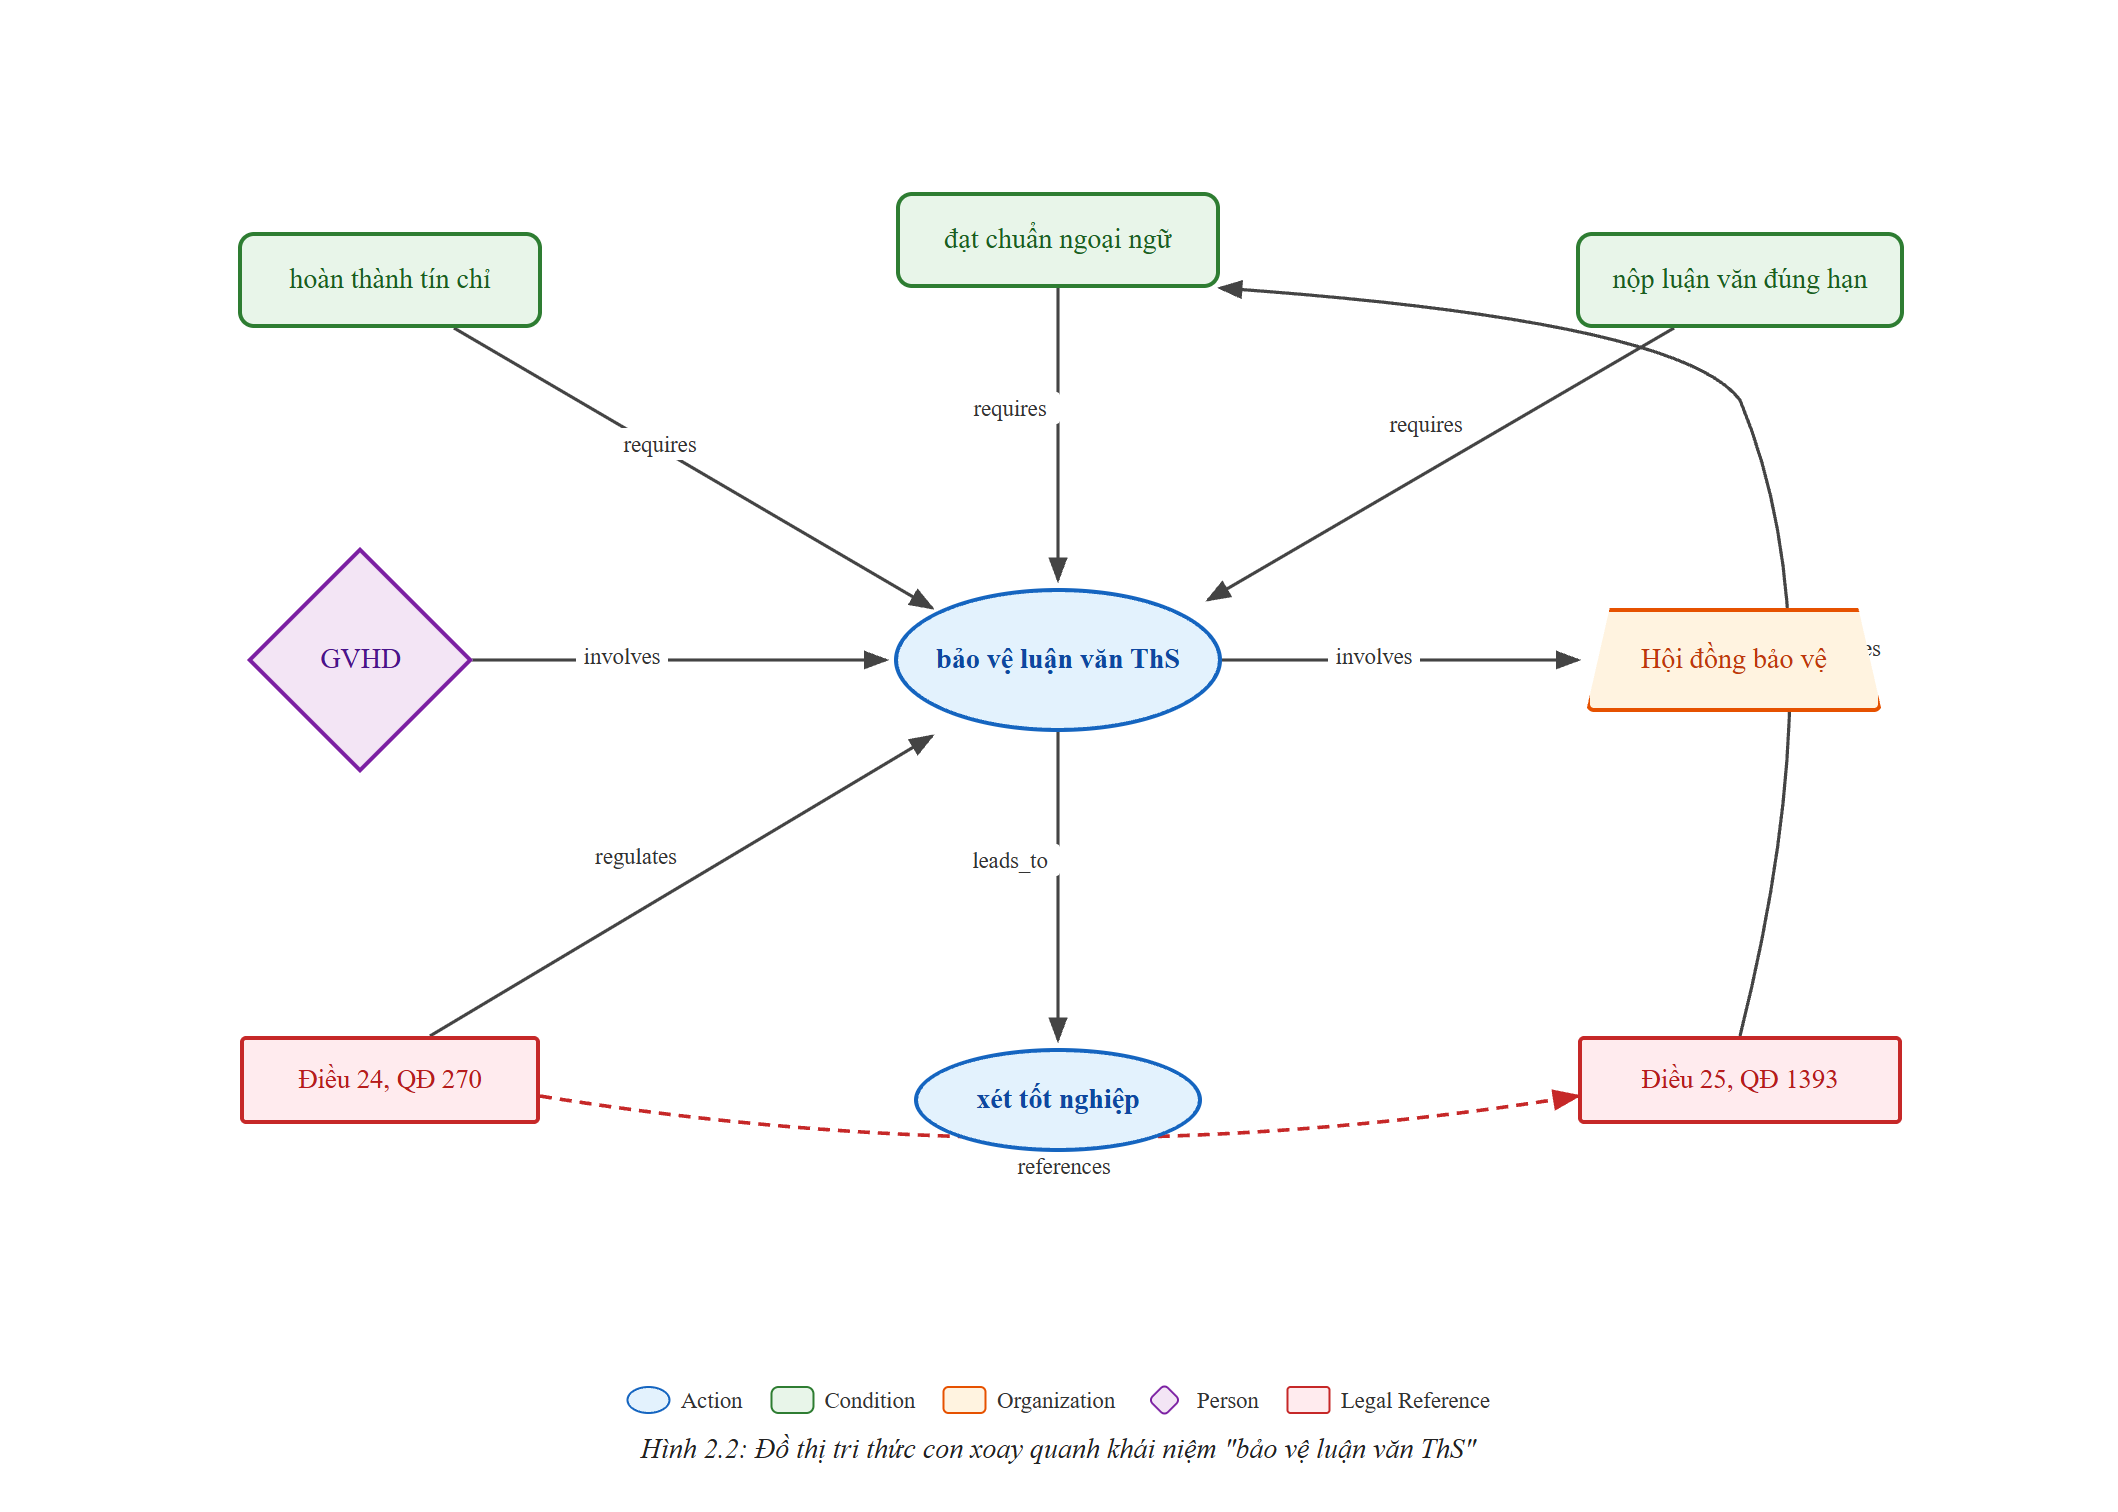
\includegraphics[width=0.95\textwidth]{graphics/figure2-2-kg-subgraph.png}
    \caption{Đồ thị con minh họa Knowledge Graph xoay quanh khái niệm \textit{``bảo vệ luận văn thạc sĩ''}. Hình elip xanh: Hành động; Hình chữ nhật bo góc xanh lá: Điều kiện; Hình thang cam: Tổ chức; Hình thoi tím: Người; Hình chữ nhật đỏ: Tham chiếu pháp lý.}
    \label{fig:kg_subgraph}
\end{figure}

% ------------------------------------------------------------
\subsection{Phân loại chủ đề}
\label{subsec:phanloa_chude}

Nội dung các quy chế đào tạo thạc sĩ được phân loại thành bảy chủ đề chính phục vụ cho việc định tuyến ý định và tổ chức Knowledge Graph. Bảng~\ref{tab:chude_phanloa} trình bày chi tiết bảy chủ đề cùng các từ khóa đặc trưng.

\begin{table}[htbp]
    \centering
    \caption{Phân loại chủ đề trong quy chế đào tạo thạc sĩ}
    \label{tab:chude_phanloa}
    \begin{tabular}{clp{7cm}}
        \toprule
        \textbf{STT} & \textbf{Chủ đề} & \textbf{Từ khóa đặc trưng} \\
        \midrule
        1 & Tuyển sinh và nhập học
          & điều kiện dự tuyển, hồ sơ tuyển sinh, nhập học, chỉ tiêu \\
        2 & Tổ chức đào tạo
          & chương trình học, học phần, tín chỉ, kế hoạch học tập \\
        3 & Giảng viên hướng dẫn
          & GVHD, tiêu chuẩn hướng dẫn, phân công, thay đổi GVHD \\
        4 & Luận văn thạc sĩ
          & đề tài, đề cương, viết luận văn, nộp luận văn \\
        5 & Bảo vệ và tốt nghiệp
          & hội đồng bảo vệ, điều kiện bảo vệ, xét tốt nghiệp, cấp bằng \\
        6 & Ngoại ngữ và liêm chính
          & chuẩn ngoại ngữ, chứng chỉ, đạo văn, liêm chính học thuật \\
        7 & Kỷ luật và khiếu nại
          & vi phạm, xử lý kỷ luật, thôi học, khiếu nại, phúc khảo \\
        \bottomrule
    \end{tabular}
\end{table}

% ============================================================
\section{Thu thập câu hỏi kiểm thử}
\label{sec:cau_hoi_kiem_thu}

% ------------------------------------------------------------
\subsection{Nguồn thu thập}
\label{subsec:nguon_thuthap}

Bộ câu hỏi kiểm thử được xây dựng từ hai nguồn chính:

\textbf{Miền quy định đào tạo} (130 câu hỏi): Câu hỏi được thu thập từ các diễn đàn trực tuyến, nhóm Facebook của học viên cao học UIT và ĐHQG-HCM, các buổi tư vấn tuyển sinh được ghi âm, và các thắc mắc học viên gửi đến Phòng Đào tạo Sau Đại học. Câu hỏi phản ánh nhu cầu tra cứu thực tế của học viên, từ các vấn đề cơ bản đến các tình huống phức tạp đòi hỏi kết nối nhiều điều khoản từ nhiều văn bản.

\textbf{Miền pháp luật Việt Nam} (400 câu hỏi): Câu hỏi được thu thập từ nhóm Facebook về tư vấn pháp luật, bao gồm các vấn đề thuộc lĩnh vực luật doanh nghiệp và luật giao thông đường bộ. Tập dữ liệu này phục vụ đánh giá tính tổng quát của hệ thống trên miền pháp lý mở rộng (Chương~\ref{chap:chapter4}).

% ------------------------------------------------------------
\subsection{Phân loại câu hỏi}
\label{subsec:phanloa_cauhoi}

Câu hỏi được phân loại theo độ phức tạp suy luận thành ba loại:

\begin{itemize}
    \item \textbf{Single-hop}: Câu hỏi có thể trả lời từ một điều khoản duy nhất trong một văn bản. Ví dụ: \textit{``Học viên cần bao nhiêu tín chỉ để hoàn thành chương trình thạc sĩ tại UIT?''}

    \item \textbf{Multi-hop}: Câu hỏi đòi hỏi kết nối thông tin từ nhiều điều khoản trong cùng một hoặc nhiều văn bản khác nhau. Ví dụ: \textit{``Học viên cao học nhập học năm 2022 cần đáp ứng những điều kiện gì để được bảo vệ luận văn?''} (cần kết hợp QĐ~270 và QĐ~1393).

    \item \textbf{Reasoning}: Câu hỏi đòi hỏi suy luận logic trên nhiều điều kiện, so sánh các tình huống hoặc xác định hành vi hợp lệ/vi phạm. Ví dụ: \textit{``Nếu học viên đã hết thời hạn đào tạo nhưng chưa bảo vệ luận văn, những phương án nào có thể thực hiện?''}
\end{itemize}

% ------------------------------------------------------------
\subsection{Thống kê bộ câu hỏi}
\label{subsec:thongke_cauhoi}

Bảng~\ref{tab:thongke_cauhoi} trình bày thống kê bộ câu hỏi kiểm thử miền quy định đào tạo thạc sĩ theo chủ đề và loại câu hỏi.

\begin{table}[htbp]
    \centering
    \caption{Thống kê bộ câu hỏi kiểm thử miền quy định đào tạo (tổng 130 câu)}
    \label{tab:thongke_cauhoi}
    \begin{tabular}{clccc r}
        \toprule
        \textbf{STT} & \textbf{Chủ đề}
            & \textbf{Single-hop} & \textbf{Multi-hop} & \textbf{Reasoning}
            & \textbf{Tổng (\%)} \\
        \midrule
        1 & Tuyển sinh và nhập học     & 10 &  5 &  3 & 18\,(13,8\%) \\
        2 & Tổ chức đào tạo            & 12 &  7 &  4 & 23\,(17,7\%) \\
        3 & Giảng viên hướng dẫn       &  6 &  5 &  3 & 14\,(10,8\%) \\
        4 & Luận văn thạc sĩ           &  8 &  8 &  4 & 20\,(15,4\%) \\
        5 & Bảo vệ và tốt nghiệp       &  7 & 10 &  5 & 22\,(16,9\%) \\
        6 & Ngoại ngữ và liêm chính    &  6 &  5 &  3 & 14\,(10,8\%) \\
        7 & Kỷ luật và khiếu nại       &  5 &  7 &  7 & 19\,(14,6\%) \\
        \midrule
        \multicolumn{2}{l}{\textbf{Tổng cộng}}
            & \textbf{54} & \textbf{47} & \textbf{29}
            & \textbf{130\,(100\%)} \\
        \bottomrule
    \end{tabular}
\end{table}

Bảng~\ref{tab:vidu_cauhoi} cung cấp mười câu hỏi mẫu đại diện từ bộ kiểm thử, kèm theo các điều khoản vàng (gold articles) được xác định thủ công bởi chuyên gia.

\begin{table}[htbp]
    \centering
    \caption{Ví dụ câu hỏi mẫu từ bộ kiểm thử}
    \label{tab:vidu_cauhoi}
    \begin{tabular}{p{0.4cm} p{6.2cm} p{2.0cm} p{3.6cm}}
        \toprule
        \textbf{STT} & \textbf{Câu hỏi} & \textbf{Loại} & \textbf{Gold articles} \\
        \midrule
        1 & Học viên cao học tại UIT cần hoàn thành bao nhiêu tín chỉ?
          & Single-hop & Điều 5, QĐ 270 \\
        2 & Điều kiện để được đăng ký bảo vệ luận văn thạc sĩ là gì?
          & Multi-hop & Điều 24 QĐ 270; Điều 25 QĐ 1393 \\
        3 & Học viên nhập học năm 2022 cần đạt chuẩn ngoại ngữ như thế nào?
          & Single-hop & Điều 25, QĐ 1393 \\
        4 & GVHD luận văn thạc sĩ cần đáp ứng tiêu chuẩn gì theo QĐ 218?
          & Single-hop & Điều 2, QĐ 218 \\
        5 & Hành vi đạo văn bị xử lý như thế nào tại UIT?
          & Single-hop & Điều 6, QĐ 851 \\
        6 & Học viên hết hạn 24 tháng chưa bảo vệ thì có thể xin gia hạn không?
          & Reasoning & Điều 12 QĐ 270; Điều 18 QĐ 1393 \\
        7 & Hội đồng bảo vệ luận văn ThS gồm những thành phần nào?
          & Single-hop & Điều 26, QĐ 270 \\
        8 & Nếu học viên bị đình chỉ học, điều kiện để được học lại là gì?
          & Reasoning & Điều 30 QĐ 270; Điều 22 QĐ 1393 \\
        9 & Học viên có thể thay đổi GVHD trong quá trình làm luận văn không?
          & Multi-hop & Điều 3 QĐ 218; Điều 18 QĐ 270 \\
        10 & Thủ tục nộp luận văn sau bảo vệ để được cấp bằng thạc sĩ?
           & Multi-hop & Điều 28 QĐ 270; Điều 27 QĐ 1393 \\
        \bottomrule
    \end{tabular}
\end{table}

% =====================================================================
% CHAPTER 3: Thiết kế giải thuật
% Pages 31-44 (numbered 15-28)
% Covers the 3-Tier KG-RAG algorithm design with full math derivations
% =====================================================================
\chapter{Thiết kế giải thuật}
\label{chap:thiet-ke-giai-thuat}

Chương này trình bày chi tiết kiến trúc giải thuật 3-Tier KG-RAG được đề xuất,
bao gồm phát biểu bài toán, tổng quan kiến trúc hệ thống, và ba tầng truy xuất:
duyệt cây cấu trúc hướng dẫn bởi LLM, truy xuất ngữ nghĩa hai cấp, và
Reciprocal Rank Fusion với mở rộng Knowledge Graph. Nội dung chương dựa trên
bài báo khoa học đã nộp tại hội nghị SOMET 2026 \cite{le2026threetier}.

% =====================================================================
\section{Phát biểu bài toán}
\label{sec:phat-bieu-bai-toan}

Cho tập hợp các tài liệu pháp lý được tổ chức thành một \textit{Document Forest}
(Rừng tài liệu):

\begin{equation}
  \mathcal{F} = \{T_1, T_2, \ldots, T_m\}
  \label{eq:document-forest}
\end{equation}

\noindent trong đó mỗi $T_i$ là một cây tài liệu đại diện cho một văn bản pháp lý.
Mỗi nút trong cây được gán một định danh duy nhất (node identifier) theo quy ước
phân cấp. Ví dụ, nút \texttt{59-2020-QH14:c2} ký hiệu Chương 2 của Luật
số 59/2020/QH14, còn \texttt{59-2020-QH14:d5} ký hiệu Điều 5 của văn bản đó.

Bài toán được phát biểu như sau: cho một truy vấn người dùng $q$, hệ thống cần
truy xuất $k$ điều khoản (articles) liên quan nhất từ $\mathcal{F}$, đồng thời
đảm bảo độ chính xác và khả năng giải thích kết quả.

% =====================================================================
\section{Tổng quan kiến trúc hệ thống}
\label{sec:tong-quan-kien-truc}

Hệ thống 3-Tier KG-RAG được thiết kế theo kiến trúc hai pha: pha ngoại tuyến
(offline) xây dựng các cấu trúc dữ liệu hỗ trợ, và pha trực tuyến (online)
thực hiện truy xuất theo ba tầng.

\begin{figure}[htbp]
  \centering
  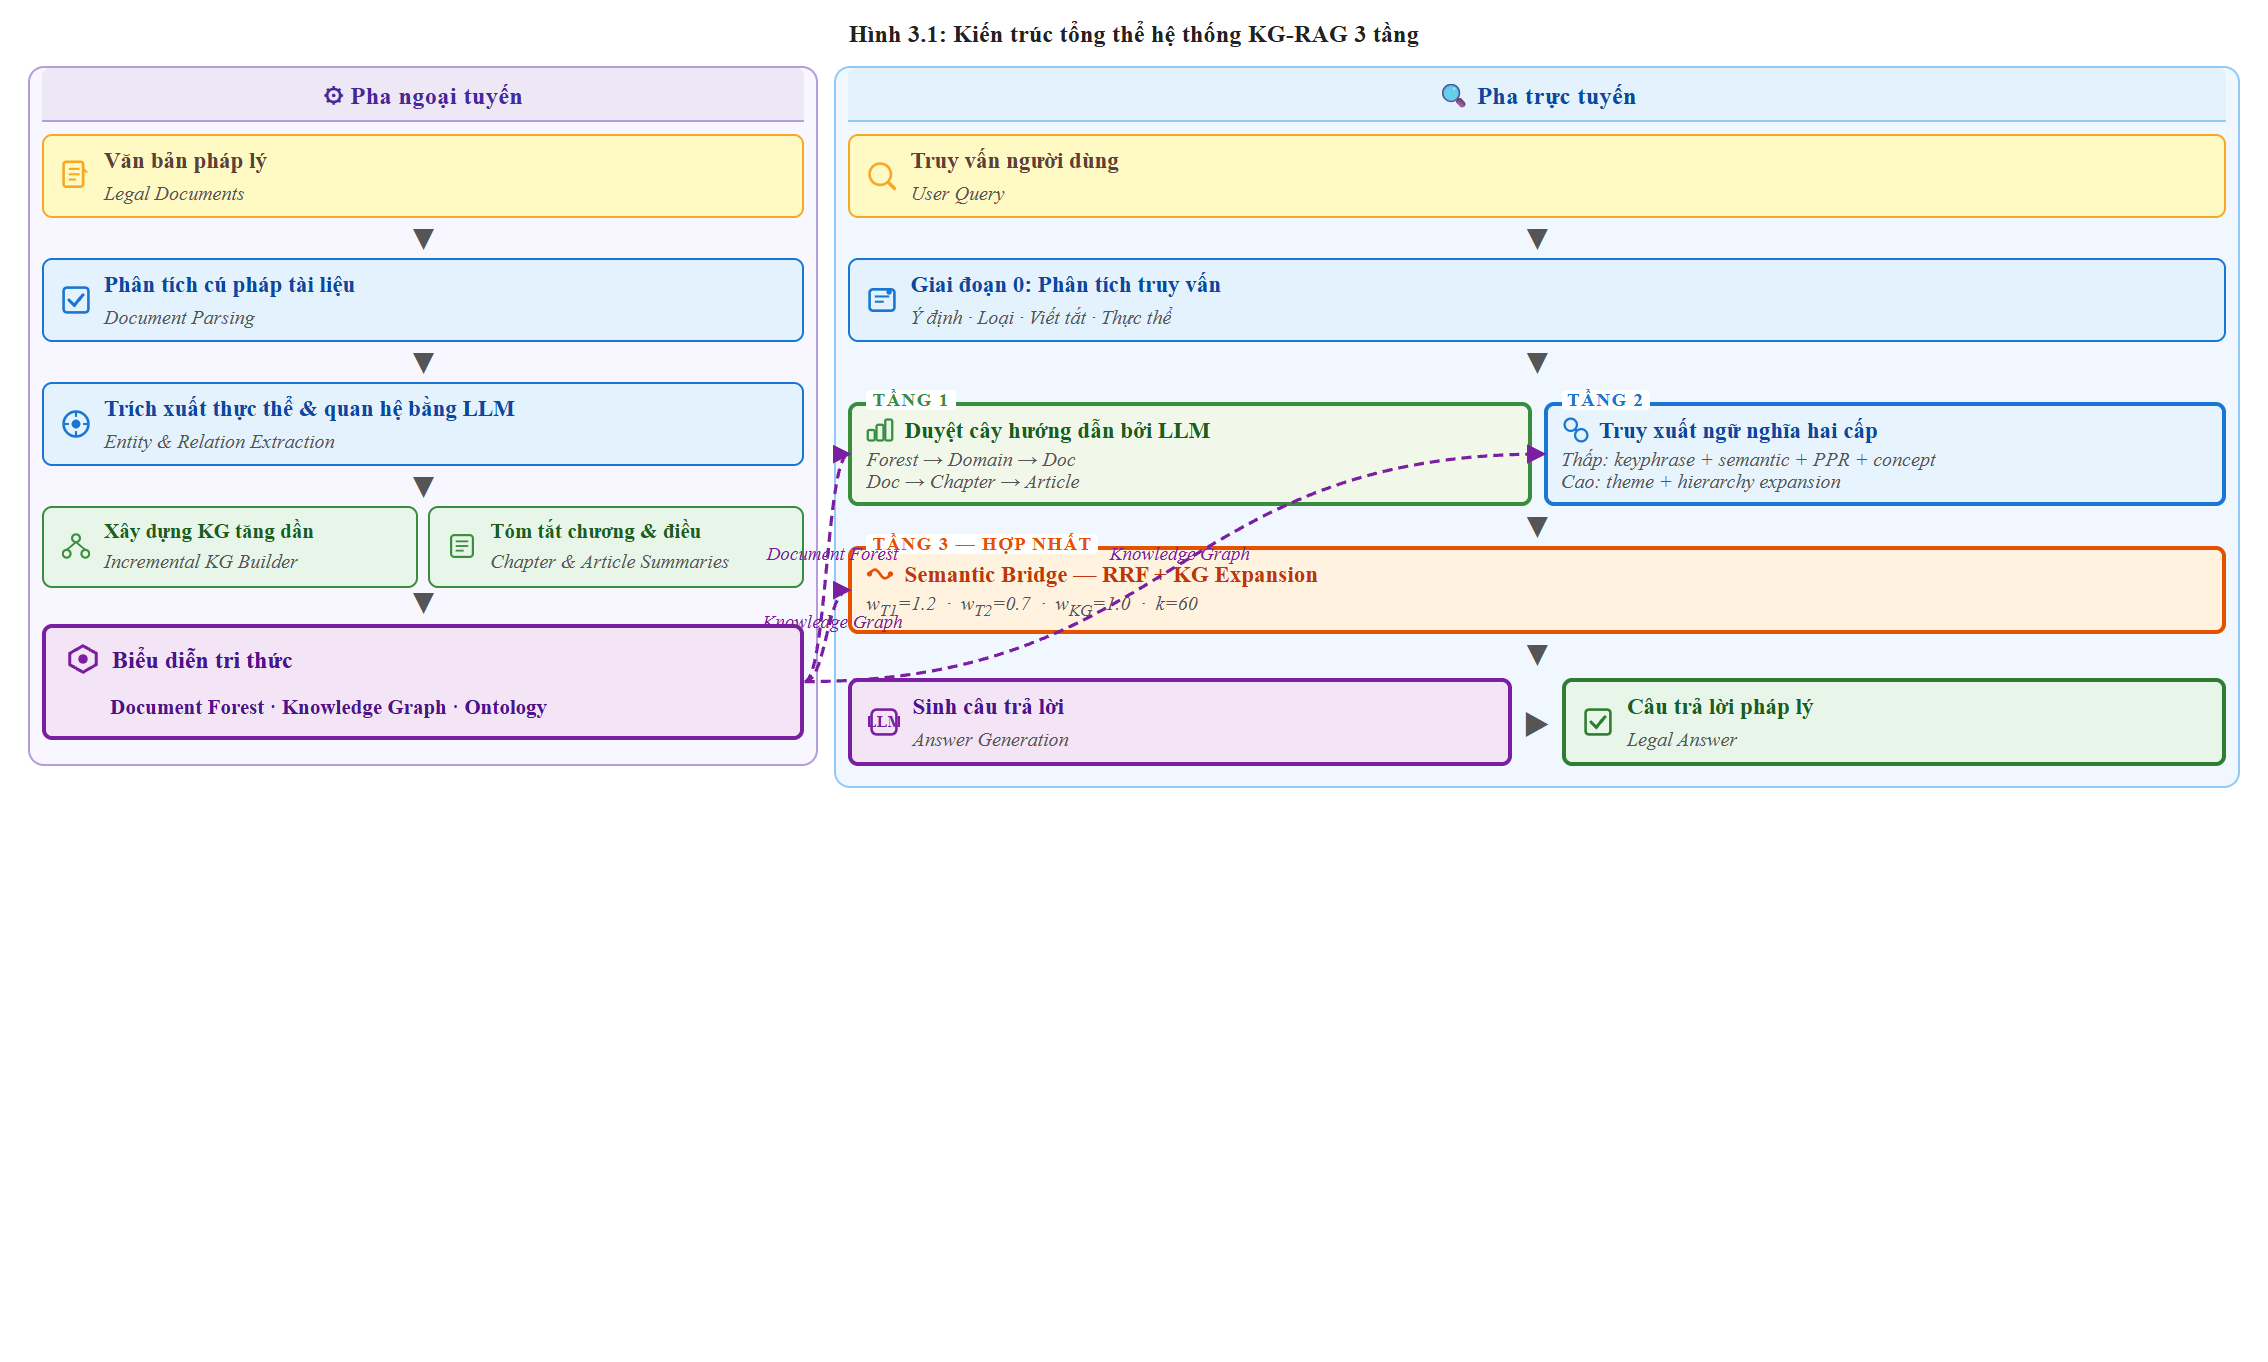
\includegraphics[width=\textwidth]{graphics/figure3-1-system-architecture.png}
  \caption{Kiến trúc hệ thống truy xuất ba tầng}
  \label{fig:kien-truc-he-thong}
\end{figure}

% -------------------------------------------------------------------
\subsection{Pha ngoại tuyến}
\label{subsec:pha-ngoai-tuyen}

\textbf{Xây dựng Document Forest.}
Mỗi tài liệu pháp lý được phân tích cú pháp và biểu diễn dưới dạng cây phân
cấp. Các nút trong cây được đặt tên theo quy tắc thống nhất mô tả trong
Bảng~\ref{tab:node-identifier-rules}.

\begin{table}[htbp]
  \centering
  \caption{Quy tắc đặt định danh nút trong Document Forest}
  \label{tab:node-identifier-rules}
  \begin{tabular}{lll}
    \toprule
    \textbf{Cấp} & \textbf{Pattern} & \textbf{Ví dụ} \\
    \midrule
    Văn bản & \texttt{\{doc\_id\}}               & \texttt{270-QĐ-ĐHCNTT} \\
    Chương  & \texttt{\{doc\_id\}:c\{N\}}         & \texttt{270:c1} \\
    Mục     & \texttt{\{doc\_id\}:s\{N\}}         & \texttt{1393:s1} \\
    Điều    & \texttt{\{doc\_id\}:d\{N\}}         & \texttt{270:d5} \\
    Khoản   & \texttt{\{doc\_id\}:d\{N\}k\{M\}}  & \texttt{270:d24k1} \\
    Điểm    & \texttt{\{doc\_id\}:d\{N\}k\{M\}p\{L\}} & \texttt{270:d24k3pa} \\
    \bottomrule
  \end{tabular}
\end{table}

\textbf{Xây dựng Summary Tree.}
Để hỗ trợ duyệt cây ở tầng 1, mỗi nút cấp văn bản, chương và mục được tóm tắt
tự động bằng mô hình Claude 3.5 Haiku. Các bản tóm tắt này cho phép LLM đánh
giá mức độ liên quan của từng nhánh cây mà không cần đọc toàn bộ nội dung.

\textbf{Xây dựng Knowledge Graph.}
Knowledge Graph (KG) được xây dựng theo quy trình bán tự động kết hợp LLM và
chuyên gia (expert-in-the-loop). Ontology sử dụng 14 loại thực thể được định
nghĩa theo chuẩn OWL với hệ thống phân cấp 4 cấp và ánh xạ nhãn tiếng Việt.
Thống kê KG được trình bày trong Bảng~\ref{tab:kg-statistics}.

\begin{table}[htbp]
  \centering
  \caption{Thống kê Knowledge Graph}
  \label{tab:kg-statistics}
  \begin{tabular}{lr}
    \toprule
    \textbf{Thành phần} & \textbf{Số lượng} \\
    \midrule
    Thực thể (entities)     & 5.936 \\
    Quan hệ (relationships) & 5.963 \\
    Loại quan hệ            & 56 \\
    Nút Document Forest     & 9.226 \\
    Tài liệu                & 13 \\
    \bottomrule
  \end{tabular}
\end{table}

% -------------------------------------------------------------------
\subsection{Pha trực tuyến}
\label{subsec:pha-truc-tuyen}

Trong pha trực tuyến, hệ thống xử lý truy vấn người dùng $q$ qua ba tầng liên
tiếp:

\begin{enumerate}
  \item \textbf{Tầng 1 -- Duyệt cây cấu trúc hướng dẫn bởi LLM:} LLM phân tích
        truy vấn và duyệt Document Forest từ gốc xuống lá, lọc ra tập ứng viên
        $C_1$ ở cấp điều.

  \item \textbf{Tầng 2 -- Truy xuất ngữ nghĩa hai cấp:} Kết hợp các tín hiệu
        ngữ nghĩa cấp thấp (keyphrase, cosine similarity, Personalized PageRank,
        concept matching) và cấp cao (theme matching, hierarchy expansion) để
        tạo tập ứng viên $C_2$.

  \item \textbf{Tầng 3 -- Hợp nhất RRF với mở rộng Knowledge Graph:} Áp dụng
        Reciprocal Rank Fusion trên $C_1$, $C_2$, và tập mở rộng từ KG để tạo
        danh sách kết quả cuối cùng.
\end{enumerate}

% =====================================================================
\section{Phân tích truy vấn}
\label{sec:phan-tich-truy-van}

Trước khi đưa truy vấn vào ba tầng truy xuất, hệ thống phân loại truy vấn thành
một trong ba loại để điều chỉnh chiến lược xử lý phù hợp:

\begin{itemize}
  \item \textbf{Keyword} (Từ khóa): Truy vấn ngắn, chứa thuật ngữ pháp lý cụ
        thể. Ví dụ: \textit{``điều kiện bảo vệ luận văn''}.

  \item \textbf{Specific} (Cụ thể): Truy vấn có ngữ cảnh rõ ràng, hỏi về một
        quy định hoặc thủ tục xác định. Ví dụ: \textit{``Học viên cần nộp hồ sơ
        gì để đăng ký bảo vệ luận văn thạc sĩ?''}.

  \item \textbf{Analytical} (Phân tích): Truy vấn mở, yêu cầu tổng hợp thông
        tin từ nhiều điều khoản hoặc so sánh quy định. Ví dụ: \textit{``So sánh
        điều kiện tốt nghiệp giữa hệ chính quy và hệ liên kết đào tạo''}.
\end{itemize}

Loại truy vấn ảnh hưởng đến trọng số của các tầng trong bước hợp nhất ở
Tầng 3 (xem Mục~\ref{sec:tang3-rrf}).

% =====================================================================
\section{Tầng 1: Duyệt cây cấu trúc hướng dẫn bởi LLM}
\label{sec:tang1-duyet-cay}

Tầng 1 sử dụng LLM để duyệt Document Forest theo chiến lược từ trên xuống
(top-down), loại bỏ sớm các nhánh không liên quan và giữ lại các ứng viên có
tiềm năng. Nhiệt độ sinh văn bản của LLM được đặt $T=0.0$ để đảm bảo tính xác
định (deterministic) trong quá trình lọc.

Quá trình duyệt cây được chia thành ba vòng lặp (loops):

\textbf{Loop 0 -- Chọn tài liệu.}
LLM nhận tóm tắt cấp văn bản của tất cả $m$ tài liệu trong $\mathcal{F}$ và
chọn ra tập con các tài liệu liên quan đến truy vấn $q$. Các tài liệu được
chọn đưa vào Loop 1.

\textbf{Loop 1 -- Chọn chương.}
Với mỗi tài liệu được chọn ở Loop 0, LLM đọc tóm tắt cấp chương và quyết định
duyệt tiếp những chương nào. Điểm ngữ nghĩa (semantic rank) được tính giữa
embedding của truy vấn và embedding của tóm tắt chương nhằm tăng cường độ chính
xác của quyết định chọn lọc.

\textbf{Loop 2 -- Chọn điều.}
Trong mỗi chương được chọn, LLM đánh giá từng điều khoản và xếp hạng chúng
theo mức độ liên quan. Ngoài điểm ngữ nghĩa đơn thuần, hệ thống áp dụng
\textit{dual rank boosting}: kết hợp cả điểm ngữ nghĩa (semantic rank) và điểm
thứ hạng kép (dual rank) để ưu tiên các điều khoản vừa liên quan về mặt ngữ
nghĩa vừa được LLM đánh giá cao.

\begin{figure}[htbp]
  \centering
  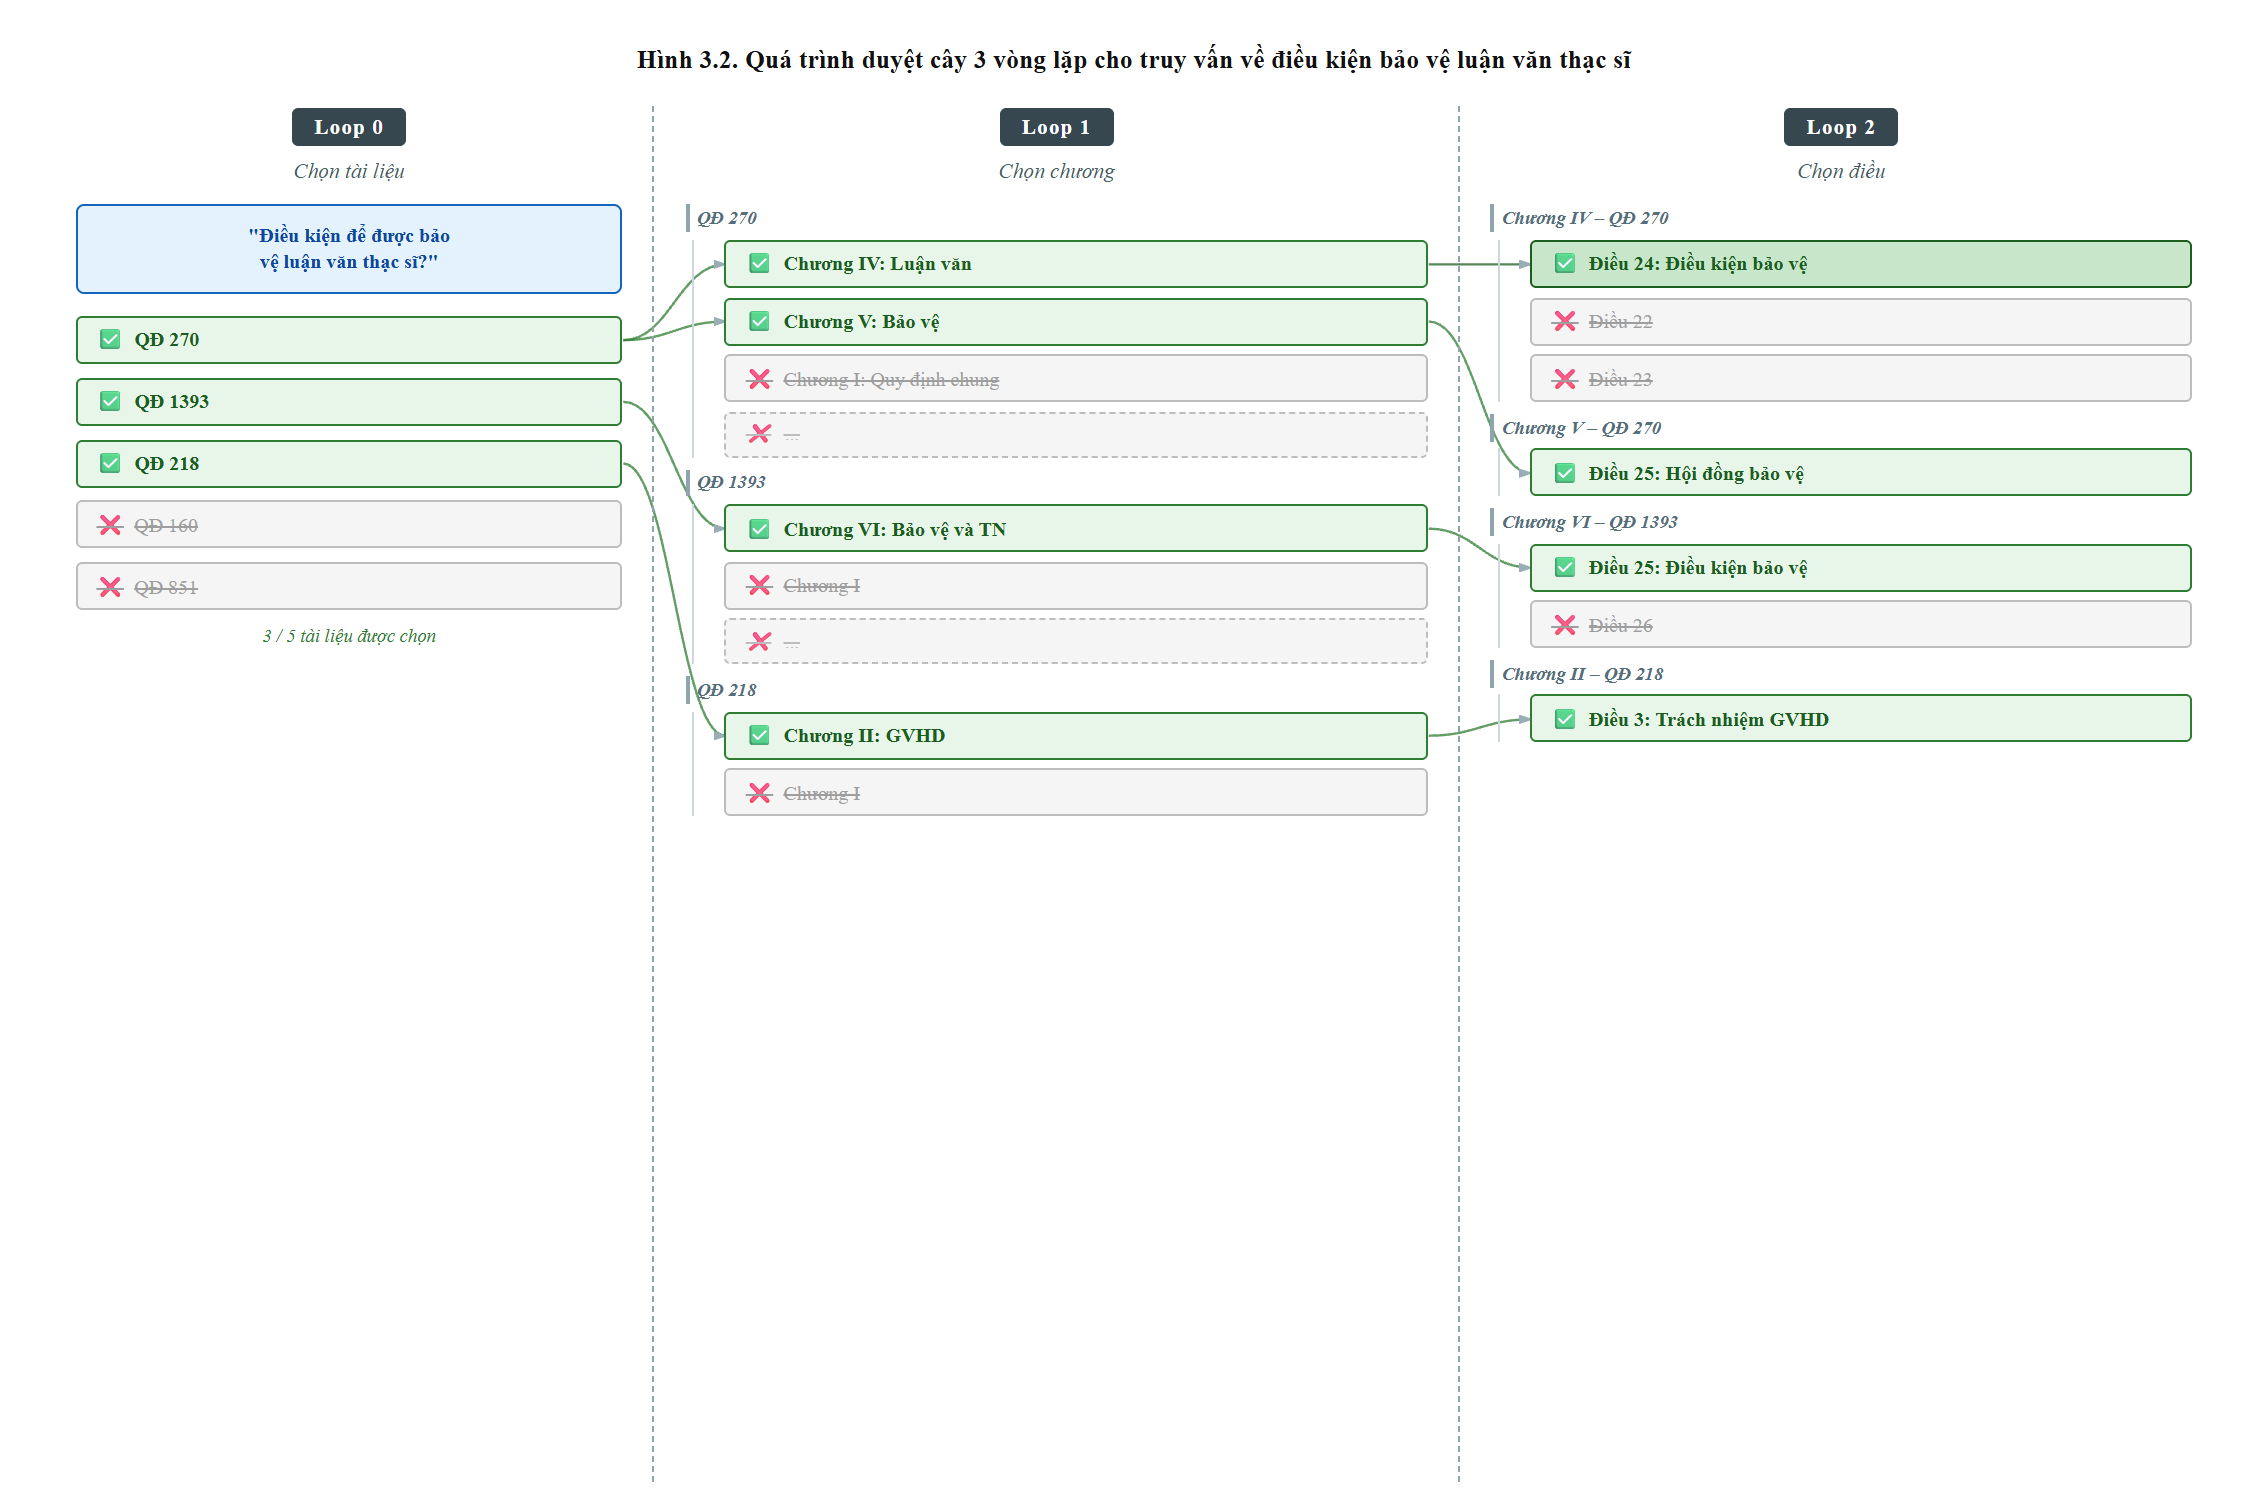
\includegraphics[width=\textwidth]{graphics/figure3-2-tree-traversal.png}
  \caption{Minh họa quá trình duyệt cây ba vòng lặp}
  \label{fig:tree-traversal}
\end{figure}

Kết quả của Tầng 1 là tập ứng viên $C_1 \subseteq \mathcal{F}$ gồm các điều
khoản được LLM xác nhận có liên quan đến truy vấn $q$.

% =====================================================================
\section{Tầng 2: Truy xuất ngữ nghĩa hai cấp}
\label{sec:tang2-semantic}

Tầng 2 tính điểm liên quan cho mỗi điều khoản ứng viên bằng cách kết hợp các
tín hiệu ngữ nghĩa ở hai cấp độ: cấp thấp (low-level, tập trung vào thực thể
và nội dung cụ thể) và cấp cao (high-level, tập trung vào chủ đề và cấu trúc
phân cấp).

% -------------------------------------------------------------------
\subsection{Truy xuất cấp thấp (Entity-specific)}
\label{subsec:low-level}

Điểm cấp thấp $s_\text{low}(a)$ cho điều khoản $a$ được tổng hợp từ bốn tín
hiệu:

\subsubsection*{1. Keyphrase Matching (Khớp cụm từ khóa)}

Hệ thống trích xuất tập thực thể $E_a$ từ điều khoản $a$ thông qua Knowledge
Graph và so khớp với các cụm từ khóa được nhận dạng từ truy vấn $q$. Điểm
keyphrase được tính như sau:

\begin{equation}
  s_\text{kp}(a) = \max_{i} (s_i) + \log(1 + n) \cdot \bar{s}
  \label{eq:keyphrase-score}
\end{equation}

\noindent trong đó $s_i$ là điểm khớp của thực thể thứ $i$ trong $E_a$, $n$ là
số lượng thực thể có điểm dương (positive entities), và $\bar{s}$ là điểm trung
bình của tất cả thực thể trong $E_a$. Thành phần logarithm $\log(1+n)$ thưởng
điểm cho các điều khoản có nhiều thực thể liên quan, thể hiện độ bao phủ chủ
đề.

\subsubsection*{2. Semantic Similarity (Tương đồng ngữ nghĩa)}

Điểm tương đồng ngữ nghĩa $s_\text{sem}(a)$ được tính bằng độ tương đồng
cosine giữa vector embedding của truy vấn $q$ và vector embedding của điều khoản
$a$, sử dụng mô hình MiniLM-L12-v2 \cite{reimers2019sbert}:

\begin{equation}
  s_\text{sem}(a) = \cos\!\left(\mathbf{e}_q,\, \mathbf{e}_a\right)
                  = \frac{\mathbf{e}_q \cdot \mathbf{e}_a}
                         {\|\mathbf{e}_q\| \cdot \|\mathbf{e}_a\|}
  \label{eq:semantic-similarity}
\end{equation}

\subsubsection*{3. Intent-aware Personalized PageRank (PPR)}

Để khai thác cấu trúc đồ thị của Knowledge Graph, hệ thống thực hiện Personalized
PageRank \cite{haveliwala2002ppr} có điều chỉnh theo ý định truy vấn. Giá trị
PPR của nút $v$ được tính theo công thức lặp:

\begin{equation}
  \text{PPR}(v) = (1-\alpha)\sum_{u \in \mathcal{N}(v)}
                  \frac{w(u,v) \cdot \text{PPR}(u)}{d(u)}
                  + \alpha \cdot p(v)
  \label{eq:ppr}
\end{equation}

\noindent trong đó:
\begin{itemize}
  \item $\alpha = 0.15$ là xác suất teleport (teleport probability),
  \item $\mathcal{N}(v)$ là tập các nút láng giềng của $v$ trong KG,
  \item $w(u,v)$ là trọng số cạnh được điều chỉnh theo ý định truy vấn
        (intent-adjusted edge weight),
  \item $d(u) = \sum_{v'} w(u,v')$ là bậc ra có trọng số (weighted out-degree)
        của nút $u$,
  \item $p(v)$ là vector cá nhân hóa (personalization vector), được thiết lập
        cao hơn tại các nút thực thể liên quan trực tiếp đến truy vấn $q$.
\end{itemize}

\subsubsection*{4. Concept Matching (Khớp khái niệm)}

Điểm khớp khái niệm đánh giá mức độ phủ của các khái niệm trọng tâm trong
điều khoản $a$ so với các khái niệm được truy vấn $q$ đề cập:

\begin{equation}
  s_\text{con}(a) = \min\!\left(1,\;
    \frac{\displaystyle\sum_{e \in E_a} w_\text{type}\!\left(\text{type}(e)\right)}
         {|E_a|}
  \right)
  \label{eq:concept-score}
\end{equation}

\noindent trong đó $w_\text{type}(\cdot)$ là trọng số gán theo loại thực thể
(entity type), phản ánh mức độ quan trọng của từng loại thực thể đối với bài
toán truy vấn pháp lý.

\subsubsection*{Tổng hợp điểm cấp thấp}

Bốn tín hiệu trên được kết hợp bằng tổng có trọng số:

\begin{equation}
  s_\text{low}(a) = w_\text{kp} \cdot s_\text{kp}(a)
                  + w_\text{sem} \cdot s_\text{sem}(a)
                  + w_\text{ppr} \cdot s_\text{ppr}(a)
                  + w_\text{con} \cdot s_\text{con}(a)
  \label{eq:low-level-combined}
\end{equation}

\noindent với các trọng số: $w_\text{kp} = 0.05$, $w_\text{sem} = 0.20$,
$w_\text{ppr} = 0.25$, $w_\text{con} = 0.20$.

% -------------------------------------------------------------------
\subsection{Truy xuất cấp cao (Conceptual)}
\label{subsec:high-level}

\subsubsection*{1. Theme Matching (Khớp chủ đề)}

Trong pha ngoại tuyến, toàn bộ các điều khoản trong $\mathcal{F}$ được phân cụm
thành các nhóm chủ đề bằng thuật toán phân cụm. Trong pha trực tuyến, truy vấn
$q$ được so khớp với top-10 cụm gần nhất theo không gian embedding. Điểm chủ đề
$s_\text{theme}(a)$ của điều khoản $a$ phản ánh mức độ gần gũi của $a$ với cụm
chủ đề phù hợp nhất với truy vấn.

\subsubsection*{2. Hierarchy Expansion (Mở rộng phân cấp)}

Điểm phân cấp $s_\text{hier}(a)$ được lan truyền từ nút cha xuống các nút con
theo hệ số suy giảm (decay factor) $\lambda = 0.5$. Cơ chế này cho phép tín
hiệu liên quan của một chương hoặc mục ảnh hưởng đến điểm số của các điều khoản
con, giảm thiểu bỏ sót do thông tin phân tán qua nhiều cấp phân cấp.

% -------------------------------------------------------------------
\subsection{Hợp nhất điểm Low-level và High-level}
\label{subsec:merge-levels}

Điểm tổng hợp cuối cùng của Tầng 2 cho điều khoản $a$ là:

\begin{equation}
  s(a) = 0.70 \cdot s_\text{low}(a)
        + 0.15 \cdot s_\text{theme}(a)
        + 0.15 \cdot s_\text{hier}(a)
  \label{eq:tier2-final-score}
\end{equation}

Các điều khoản có điểm $s(a) < 0.1$ bị loại khỏi tập ứng viên. Tập ứng viên
còn lại sau bước lọc này tạo thành $C_2$.

% =====================================================================
\section{Tầng 3: Hợp nhất RRF với mở rộng Knowledge Graph}
\label{sec:tang3-rrf}

% -------------------------------------------------------------------
\subsection{Mở rộng Knowledge Graph}
\label{subsec:kg-expansion}

Trước khi thực hiện hợp nhất, hệ thống sử dụng KG để mở rộng tập ứng viên bằng
cách bổ sung các điều khoản liên quan nhưng chưa xuất hiện trong $C_1$ hoặc
$C_2$. Quá trình mở rộng tuân theo các ràng buộc sau:

\begin{itemize}
  \item Chỉ duyệt qua các loại quan hệ \textit{mạnh} (STRONG relations):
        \texttt{references}, \texttt{requires}, \texttt{depends\_on}.

  \item \textbf{Giới hạn liên chương:} Với mỗi điều khoản nguồn, tối đa 5 điều
        khoản từ chương khác được thêm vào.

  \item \textbf{Giới hạn cùng chương:} Tối đa 2 điều khoản từ cùng chương được
        thêm vào.

  \item \textbf{Lọc ngữ nghĩa:} Chỉ giữ lại điều khoản mở rộng có độ tương đồng
        cosine với truy vấn $q$ đạt ngưỡng $\cos(\mathbf{e}_q, \mathbf{e}_a)
        \geq 0.4$.
\end{itemize}

Tập điều khoản mở rộng từ KG được ký hiệu là $C_\text{KG}$.

% -------------------------------------------------------------------
\subsection{Reciprocal Rank Fusion}
\label{subsec:rrf}

Hệ thống áp dụng Reciprocal Rank Fusion (RRF) \cite{cormack2009rrf} để hợp nhất
ba danh sách xếp hạng: $C_1$ (Tầng 1), $C_2$ (Tầng 2), và $C_\text{KG}$ (mở
rộng KG). Điểm RRF của điều khoản $d$ được tính như sau:

\begin{equation}
  \text{RRF}(d) = \sum_{s \in \{T_1,\, T_2,\, \text{KG}\}}
                  w_s \cdot \frac{1}{k + \text{rank}_s(d)}
  \label{eq:rrf}
\end{equation}

\noindent trong đó:
\begin{itemize}
  \item $k = 60$ là hằng số làm mịn (smoothing constant) theo đề xuất gốc
        \cite{cormack2009rrf},
  \item $\text{rank}_s(d)$ là thứ hạng của tài liệu $d$ trong danh sách $s$
        (bằng $+\infty$ nếu $d$ không xuất hiện trong $s$),
  \item $w_{T_1} = 1.2$, $w_{T_2} = 0.7$, $w_\text{KG} = 1.0$ là trọng số
        của từng nguồn xếp hạng.
\end{itemize}

\begin{figure}[htbp]
  \centering
  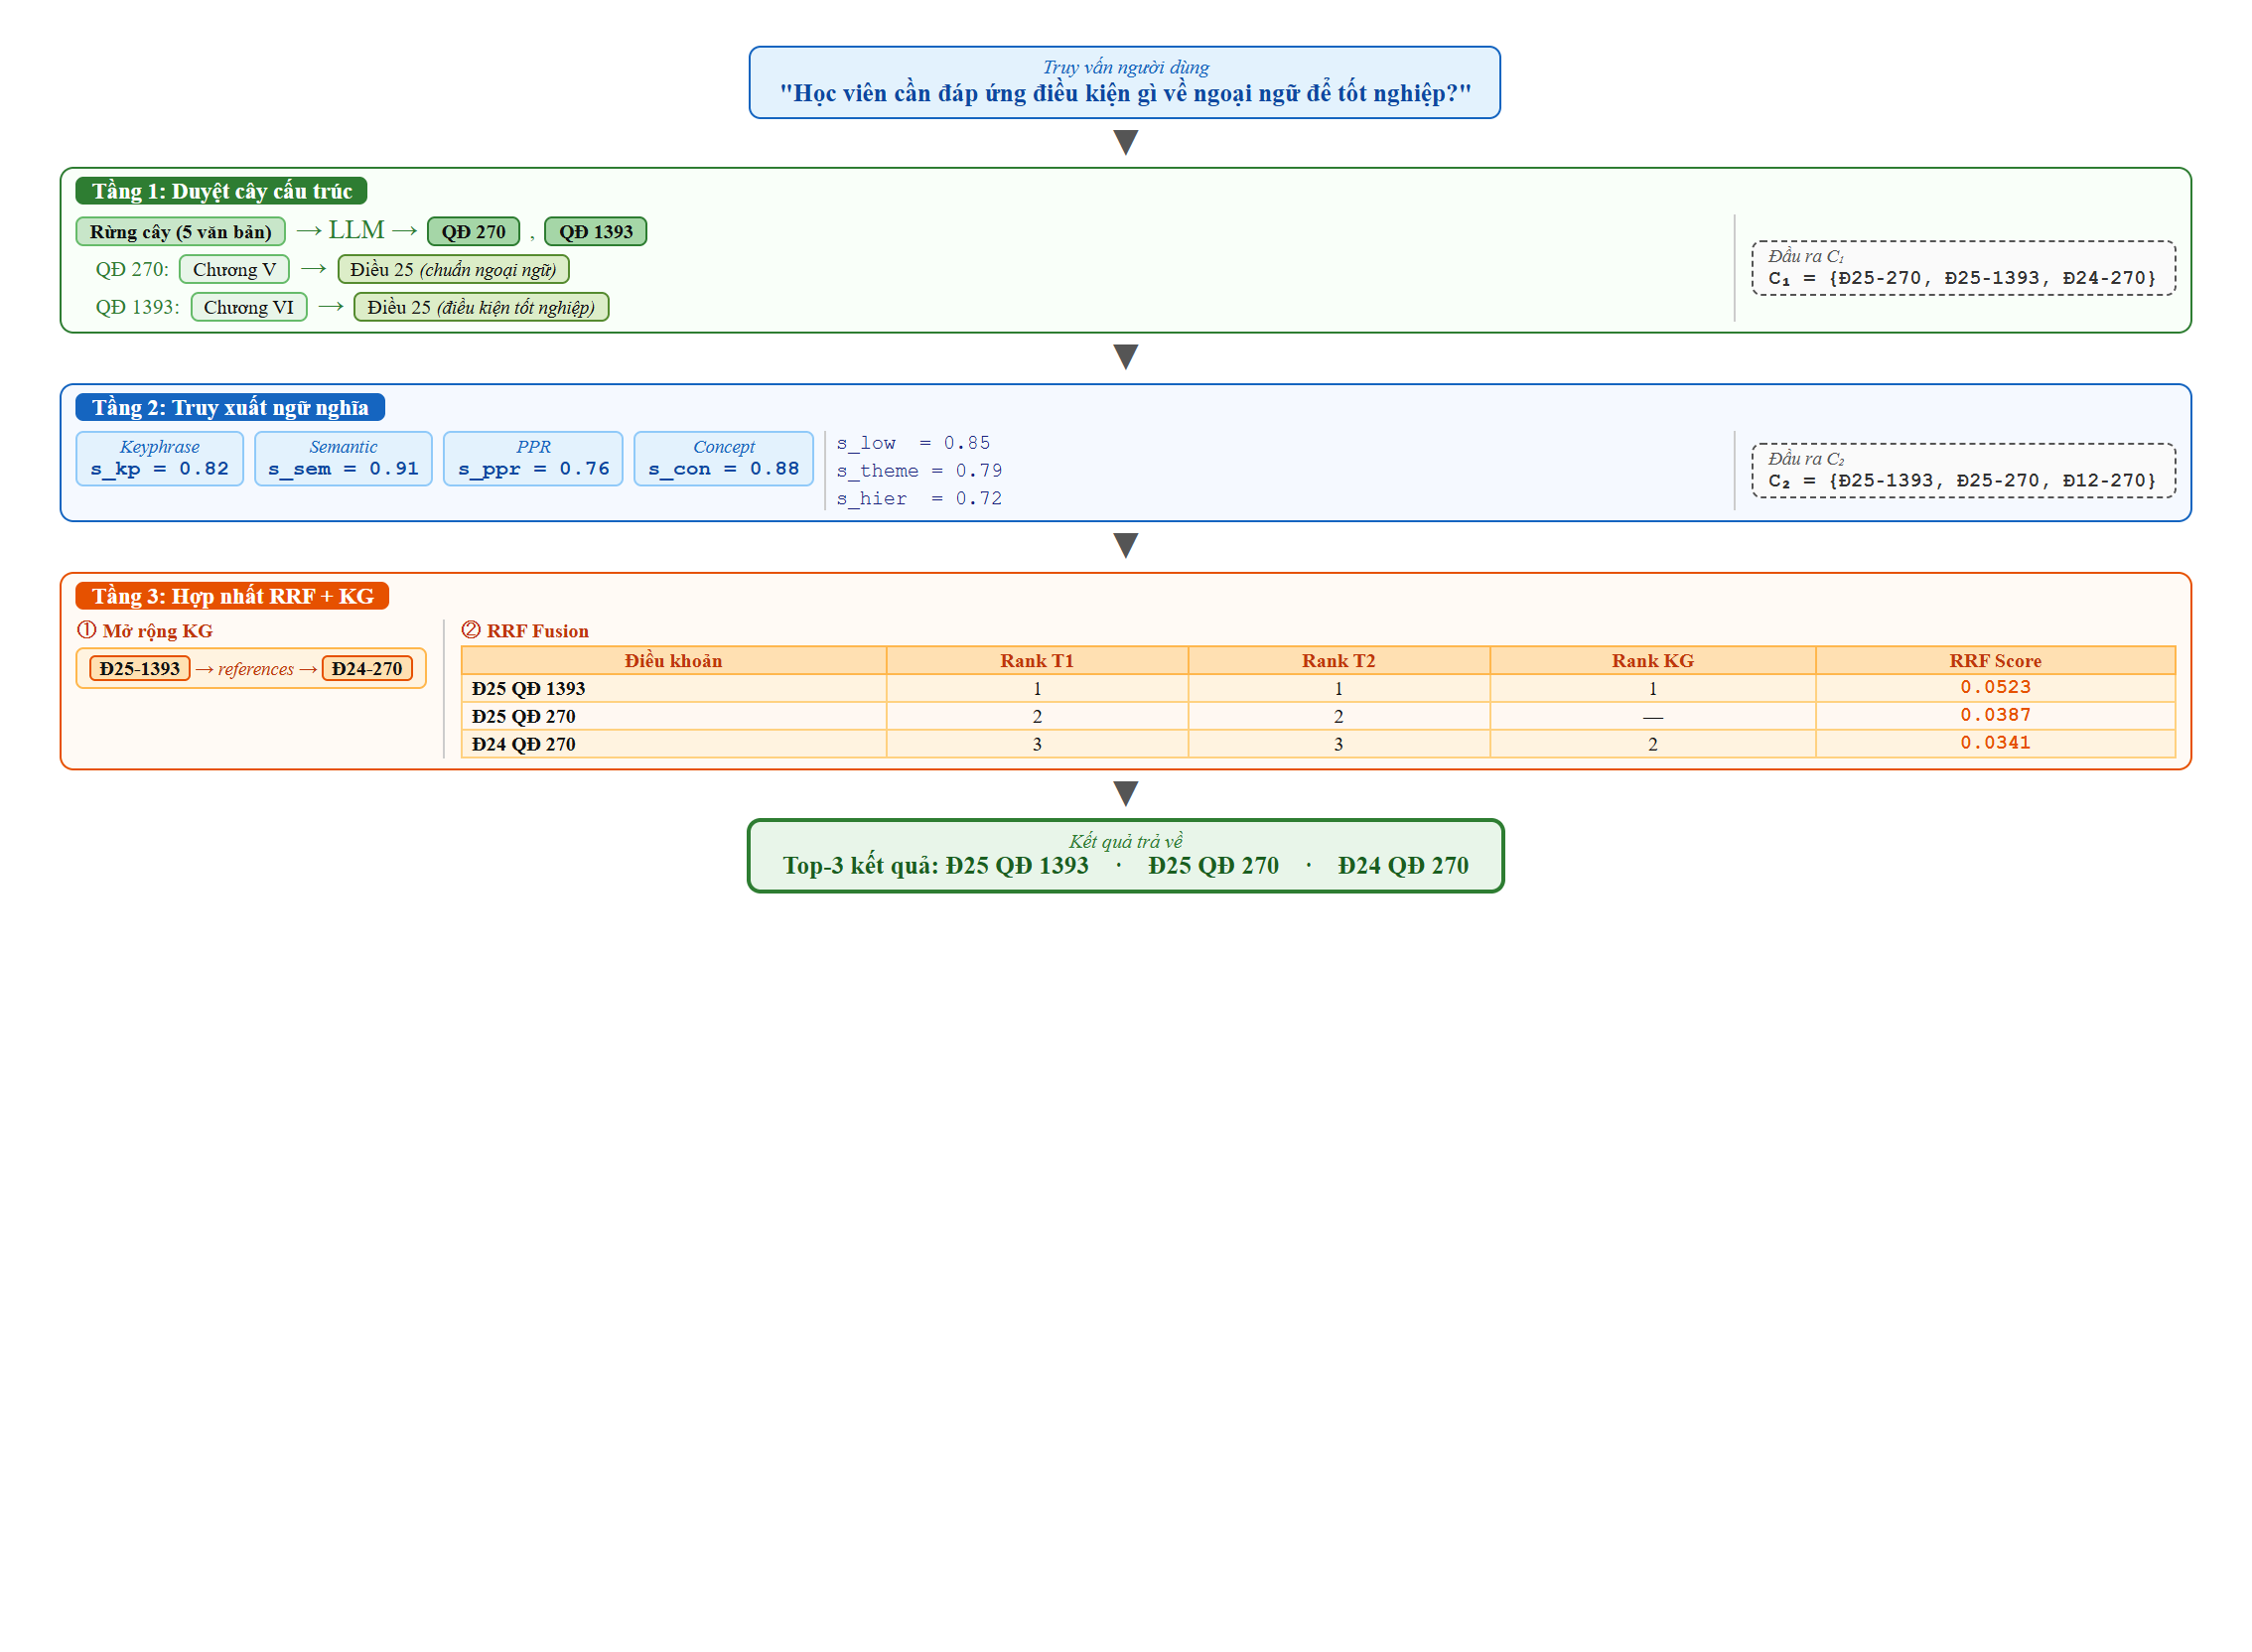
\includegraphics[width=\textwidth]{graphics/figure3-3-end-to-end-flow.png}
  \caption{Luồng xử lý end-to-end cho truy vấn điều kiện ngoại ngữ tốt nghiệp}
  \label{fig:end-to-end-flow}
\end{figure}

% -------------------------------------------------------------------
\subsection{Các cơ chế điều chỉnh}
\label{subsec:dieu-chinh}

Ngoài công thức RRF cơ bản, hệ thống áp dụng ba cơ chế điều chỉnh để nâng cao
chất lượng kết quả:

\subsubsection*{1. Dynamic Tree Weight (Trọng số cây động)}

Tầng 1 (duyệt cây) có hiệu quả thấp hơn khi truy vấn mang tính khái quát hoặc
LLM trả về phần lớn các điều khoản chung chung. Do đó, hệ thống áp dụng cơ chế
điều chỉnh trọng số động: nếu $\geq 50\%$ các điều khoản trong $C_1$ được phát
hiện là mang tính khái quát (generic), trọng số của Tầng 1 được giảm từ
$w_{T_1} = 1.2$ xuống $w_{T_1} = 0.7$, đồng thời trọng số KG được tăng từ
$w_\text{KG} = 1.0$ lên $w_\text{KG} = 1.3$.

\subsubsection*{2. Penalty (Hình phạt điểm)}

Các điều khoản thuộc các nhóm đặc biệt bị áp dụng hệ số hình phạt nhân vào điểm
RRF:

\begin{itemize}
  \item \textbf{Procedural} (Thủ tục hành chính): hệ số $\times 0.35$ — các điều
        khoản chỉ mô tả quy trình nộp hồ sơ, thời hạn hành chính, thường ít
        liên quan đến nội dung câu trả lời.
  \item \textbf{Noise} (Nhiễu): hệ số $\times 0.20$ — các điều khoản được xác
        định là không liên quan đến miền kiến thức của truy vấn.
  \item \textbf{Generic} (Khái quát): hệ số $\times 0.15$ — các điều khoản quá
        chung chung, không cung cấp thông tin cụ thể.
\end{itemize}

\subsubsection*{3. Agreement Bonus (Thưởng đồng thuận)}

Một điều khoản xuất hiện đồng thời trong nhiều tầng chứng tỏ sự đồng thuận
(agreement) từ nhiều nguồn bằng chứng độc lập, cho thấy độ tin cậy cao hơn.
Hệ thống thưởng điểm $+0.005$ cho mỗi tầng bổ sung (ngoài tầng đầu tiên) mà
điều khoản xuất hiện trong. Cụ thể, nếu một điều khoản xuất hiện trong $t \geq 2$
tầng, điểm RRF của nó được cộng thêm $(t-1) \times 0.005$.

\vspace{1em}
\noindent Danh sách kết quả cuối cùng gồm $k$ điều khoản có điểm RRF cao nhất
(sau khi áp dụng penalty và agreement bonus) được chuyển đến module sinh câu
trả lời (generation module) để tạo phản hồi cho người dùng.

\chapter{Thiết kế hệ thống và thử nghiệm}
\label{chap:chapter4}

Chương này trình bày thiết kế chi tiết hệ thống KG-RAG ba tầng, bao gồm các yêu cầu chức năng và phi chức năng, kiến trúc triển khai, kết quả thử nghiệm định lượng trên hai miền dữ liệu, phân tích lỗi, và mô tả ứng dụng minh họa chatbot tư vấn văn bản pháp luật.

% ===================================================================
\section{Yêu cầu hệ thống}
\label{sec:yeu-cau-he-thong}

\subsection{Yêu cầu chức năng}
\label{subsec:yc-chuc-nang}

Hệ thống cần đáp ứng ba yêu cầu chức năng cốt lõi:

\begin{enumerate}
  \item \textbf{Tiếp nhận truy vấn ngôn ngữ tự nhiên:} Hệ thống phải nhận câu hỏi của người dùng bằng tiếng Việt thông qua giao diện web, phân tích ý định và trích xuất các khái niệm pháp lý liên quan để phục vụ quá trình truy xuất.

  \item \textbf{Truy xuất điều khoản liên quan:} Dựa trên câu hỏi đầu vào, hệ thống phải xác định và xếp hạng các điều khoản văn bản luật hoặc quy chế đào tạo liên quan nhất thông qua kiến trúc truy xuất ba tầng, bảo đảm độ chính xác cao theo các chỉ số Hit@k và MRR.

  \item \textbf{Sinh câu trả lời có căn cứ:} Hệ thống phải tổng hợp thông tin từ các điều khoản đã truy xuất và sinh ra câu trả lời mạch lạc, có trích dẫn nguồn cụ thể, theo cấu trúc IRAC (Issue -- Rule -- Application -- Conclusion) phù hợp với từng miền kiến thức.
\end{enumerate}

\subsection{Yêu cầu phi chức năng}
\label{subsec:yc-phi-chuc-nang}

\begin{itemize}
  \item \textbf{Thời gian phản hồi:} Toàn bộ chu trình từ khi người dùng gửi câu hỏi đến khi nhận được câu trả lời phải hoàn thành trong vòng không quá 10 giây trong điều kiện vận hành thông thường.

  \item \textbf{Hỗ trợ tiếng Việt Unicode:} Hệ thống phải xử lý đúng toàn bộ ký tự tiếng Việt có dấu theo chuẩn Unicode (UTF-8), bao gồm cả trong quá trình nhúng văn bản (embedding), lập chỉ mục và sinh câu trả lời.

  \item \textbf{Giao diện thân thiện người dùng:} Giao diện web phải hoạt động tốt trên cả máy tính để bàn (desktop) lẫn thiết bị di động (mobile), có thiết kế trực quan, dễ sử dụng cho người dùng không có nền tảng kỹ thuật.
\end{itemize}

% ===================================================================
\section{Kiến trúc hệ thống}
\label{sec:kien-truc-he-thong}

\subsection{Tổng quan kiến trúc triển khai}
\label{subsec:tongquan-kientruc}

Hệ thống được thiết kế theo mô hình client--server hai lớp với tầng backend và tầng frontend tách biệt hoàn toàn, giao tiếp qua REST API.

\textbf{Backend} được xây dựng bằng Python FastAPI, đảm nhiệm toàn bộ luồng xử lý nghiệp vụ: tiếp nhận truy vấn, điều phối pipeline truy xuất ba tầng, tương tác với đồ thị tri thức, FAISS vector store và LLM để sinh câu trả lời.

\textbf{Frontend} được xây dựng bằng React 18 và TypeScript, cung cấp giao diện chat tương tác, hiển thị kết quả truy xuất kèm trích dẫn nguồn, và phản hồi trạng thái quá trình xử lý theo thời gian thực.

\subsection{Công nghệ sử dụng}
\label{subsec:cong-nghe}

Bảng~\ref{tab:cong-nghe} tóm tắt các công nghệ chính được sử dụng trong từng thành phần của hệ thống.

\begin{table}[htbp]
  \centering
  \caption{Công nghệ sử dụng trong hệ thống}
  \label{tab:cong-nghe}
  \begin{tabular}{ll}
    \toprule
    \textbf{Thành phần} & \textbf{Công nghệ} \\
    \midrule
    Backend API        & Python 3.11, FastAPI \\
    Frontend           & React 18, TypeScript, Tailwind CSS \\
    LLM                & Claude 3.5 Haiku (Anthropic) \\
    Embedding          & \texttt{sentence-transformers/all-MiniLM-L12-v2} \\
    Knowledge Graph    & NetworkX + custom graph store \\
    Vector Store       & FAISS \\
    Cơ sở dữ liệu      & SQLite (metadata), JSON (document store) \\
    Triển khai         & Docker, Nginx \\
    \bottomrule
  \end{tabular}
\end{table}

\subsection{Chi tiết triển khai}
\label{subsec:chitiet-trienkhay}

Luồng xử lý một truy vấn hoàn chỉnh diễn ra như sau. Câu hỏi của người dùng được gửi qua HTTP POST đến endpoint \texttt{/api/query} của FastAPI. Backend khởi động pipeline truy xuất ba tầng theo kiến trúc đã trình bày tại Chương~3: (i)~Tầng 1 sử dụng tóm tắt chương để lọc phạm vi; (ii)~Tầng 2 kết hợp BM25, embedding FAISS và đồ thị tri thức để xếp hạng sơ bộ; (iii)~Tầng 3 mở rộng kết quả qua PPR trên đồ thị và hợp nhất bằng RRF~\cite{cormack2009rrf}. Các điều khoản được chọn sau đó được đưa vào LLM để sinh câu trả lời theo cấu trúc IRAC. Kết quả trả về client dưới dạng JSON bao gồm câu trả lời và danh sách điều khoản nguồn.

Hệ thống được đóng gói bằng Docker Compose với hai service: \texttt{backend} (FastAPI) và \texttt{frontend} (React build được phục vụ qua Nginx). Toàn bộ đồ thị tri thức và chỉ mục FAISS được tải vào bộ nhớ khi khởi động để tối thiểu hóa độ trễ truy vấn.

% ===================================================================
\section{Kết quả thử nghiệm}
\label{sec:ket-qua-thu-nghiem}

\subsection{Các chỉ số đánh giá}
\label{subsec:chi-so-danh-gia}

Nghiên cứu sử dụng hai chỉ số định lượng tiêu chuẩn trong lĩnh vực truy xuất thông tin để đánh giá hiệu năng các hệ thống.

\textbf{Hit@k} (Tỷ lệ trúng tại vị trí k) đo lường tỷ lệ câu hỏi mà ít nhất một điều khoản vàng (gold article) xuất hiện trong danh sách $k$ kết quả truy xuất hàng đầu:
\begin{equation}
  \text{Hit@}k = \frac{1}{|Q|} \sum_{q \in Q} \mathbf{1}\!\left[\text{gold}_q \cap \text{top-}k_q \neq \emptyset\right]
  \label{eq:hitk}
\end{equation}
trong đó $Q$ là tập câu hỏi kiểm thử, $\text{gold}_q$ là tập điều khoản vàng cho câu hỏi $q$, và $\text{top-}k_q$ là $k$ điều khoản được hệ thống xếp hạng cao nhất.

\textbf{MRR} (Mean Reciprocal Rank -- Trung bình nghịch đảo thứ hạng) đo lường trung bình nghịch đảo thứ hạng của điều khoản vàng đầu tiên xuất hiện trong danh sách kết quả:
\begin{equation}
  \text{MRR} = \frac{1}{|Q|} \sum_{q \in Q} \frac{1}{\text{rank}_q}
  \label{eq:mrr}
\end{equation}
trong đó $\text{rank}_q$ là thứ hạng của điều khoản vàng xuất hiện sớm nhất cho câu hỏi $q$. MRR bằng $0$ nếu không có điều khoản vàng nào xuất hiện trong danh sách kết quả được xét.

\subsection{Các hệ thống đối sánh}
\label{subsec:he-thong-doi-sanh}

Để đánh giá khách quan, kiến trúc ba tầng được so sánh với bốn hệ thống cơ sở:

\begin{itemize}
  \item \textbf{NaiveRAG:} Kết hợp BM25 và embedding vector (all-MiniLM-L12-v2) theo phương pháp truy xuất phẳng, không sử dụng cấu trúc đồ thị hay phân cấp ngữ nghĩa.

  \item \textbf{LightRAG}~\cite{guo2025lightrag}: Hệ thống RAG tích hợp đồ thị tri thức với chiến lược truy xuất hai chế độ (local và global), sử dụng LLM để xây dựng đồ thị thực thể--quan hệ tự động.

  \item \textbf{RAPTOR}~\cite{sarthi2024raptor}: Phương pháp xây dựng cây tóm tắt phân cấp đệ quy từ văn bản nguồn, cho phép truy xuất tổng hợp ở nhiều mức độ chi tiết khác nhau.

  \item \textbf{PageIndex}~\cite{zhang2025pageindex}: Phương pháp lập chỉ mục theo trang văn bản kết hợp với chiến lược truy xuất phân cấp hai bước, tối ưu cho tài liệu có cấu trúc trang rõ ràng.
\end{itemize}

\subsection{Case Study 1: Miền pháp luật Việt Nam}
\label{subsec:casestudy-phapluat}

Bộ kiểm thử miền pháp luật gồm 400 câu hỏi, chia đều trên hai lĩnh vực: luật doanh nghiệp (200 câu) và luật giao thông đường bộ (200 câu). Các câu hỏi được xây dựng thủ công bởi người có chuyên môn pháp lý, mỗi câu hỏi có ít nhất một điều khoản vàng tương ứng.

\begin{table}[htbp]
  \centering
  \caption{Tỷ lệ Hit (\%) trên miền pháp luật (400 câu hỏi)}
  \label{tab:hit-phapluat}
  \begin{tabular}{lrrrrr}
    \toprule
    \textbf{Hệ thống} & \textbf{Hit@1} & \textbf{Hit@3} & \textbf{Hit@5} & \textbf{Hit@10} & \textbf{MRR} \\
    \midrule
    NaiveRAG            & 10{,}5 & 21{,}8 & 30{,}0 & 42{,}8 & 0{,}179 \\
    LightRAG            & 13{,}0 & 27{,}5 & 39{,}5 & 55{,}8 & 0{,}224 \\
    RAPTOR              & 12{,}2 & 23{,}2 & 31{,}2 & 41{,}0 & 0{,}196 \\
    PageIndex           & 38{,}2 & 58{,}5 & 70{,}2 & 84{,}8 & 0{,}507 \\
    \textbf{3-Tier (ours)} & \textbf{39{,}8} & \textbf{63{,}2} & \textbf{78{,}2} & \textbf{92{,}2} & \textbf{0{,}603} \\
    \bottomrule
  \end{tabular}
\end{table}

Bảng~\ref{tab:hit-phapluat} cho thấy kiến trúc ba tầng đạt Hit@10 = 92{,}2\% và MRR = 0{,}603, vượt trội so với PageIndex (84{,}8\%; 0{,}507) và các hệ thống còn lại. Đặc biệt, mức cải thiện từ Hit@1 sang Hit@10 của hệ thống ba tầng (39{,}8\% lên 92{,}2\%) cho thấy kiến trúc này có khả năng thu hồi toàn diện nhờ giai đoạn mở rộng đồ thị.

Bảng~\ref{tab:hit10-mien} phân tích chi tiết Hit@10 theo từng lĩnh vực con trong miền pháp luật.

\begin{table}[htbp]
  \centering
  \caption{Hit@10 (\%) theo miền trên ba lĩnh vực}
  \label{tab:hit10-mien}
  \begin{tabular}{lrrr}
    \toprule
    \textbf{Hệ thống} & \textbf{Doanh nghiệp (200)} & \textbf{Giao thông (200)} & \textbf{Tổng (400)} \\
    \midrule
    NaiveRAG  & 34{,}5 & 51{,}0 & 42{,}8 \\
    LightRAG  & 50{,}5 & 61{,}0 & 55{,}8 \\
    RAPTOR    & 32{,}5 & 49{,}5 & 41{,}0 \\
    PageIndex & 76{,}6 & 92{,}6 & 84{,}8 \\
    \textbf{3-Tier (ours)} & \textbf{86{,}5} & \textbf{98{,}0} & \textbf{92{,}2} \\
    \bottomrule
  \end{tabular}
\end{table}

Kết quả cho thấy lĩnh vực giao thông đường bộ có Hit@10 cao hơn đáng kể so với lĩnh vực doanh nghiệp ở tất cả các hệ thống, phản ánh sự khác biệt về độ phức tạp suy luận pháp lý giữa hai lĩnh vực.

\subsection{Case Study 2: Miền quy định đào tạo}
\label{subsec:casestudy-daotao}

Bộ kiểm thử miền quy định đào tạo gồm 130 câu hỏi được xây dựng dựa trên năm văn bản quy chế đào tạo sau đại học của Trường Đại học Công nghệ Thông tin~\cite{le2026threetier}. Bảng~\ref{tab:hit-daotao} trình bày kết quả so sánh.

\begin{table}[htbp]
  \centering
  \caption{Kết quả trên miền quy định đào tạo (130 câu hỏi)}
  \label{tab:hit-daotao}
  \begin{tabular}{lrrrrr}
    \toprule
    \textbf{Hệ thống} & \textbf{Hit@1} & \textbf{Hit@3} & \textbf{Hit@5} & \textbf{Hit@10} & \textbf{MRR} \\
    \midrule
    NaiveRAG            & 12{,}3 & 26{,}2 & 36{,}2 & 50{,}0 & 0{,}215 \\
    LightRAG            & 18{,}5 & 33{,}1 & 43{,}1 & 58{,}5 & 0{,}279 \\
    RAPTOR              & 16{,}2 & 30{,}0 & 40{,}0 & 53{,}8 & 0{,}253 \\
    PageIndex           & 33{,}1 & 50{,}0 & 59{,}2 & 74{,}6 & 0{,}438 \\
    \textbf{3-Tier (ours)} & \textbf{40{,}0} & \textbf{60{,}8} & \textbf{73{,}1} & \textbf{87{,}9} & \textbf{0{,}594} \\
    \bottomrule
  \end{tabular}
\end{table}

Kiến trúc ba tầng tiếp tục dẫn đầu với Hit@10 = 87{,}9\% và MRR = 0{,}594 trên miền đào tạo. So với miền pháp luật (Hit@10 = 92{,}2\%), hiệu năng trên miền đào tạo thấp hơn một phần do đặc thù của quy chế đào tạo có nhiều điều khoản liên quan chéo phức tạp giữa các văn bản.

\subsection{Ablation Study}
\label{subsec:ablation}

Để hiểu đóng góp của từng thành phần trong kiến trúc ba tầng, chúng tôi tiến hành ablation study bằng cách lần lượt loại bỏ hoặc vô hiệu hóa từng thành phần và đo lại chỉ số Hit@10 trung bình trên ba lần chạy độc lập.

\begin{table}[htbp]
  \centering
  \caption{Kết quả ablation study (Hit@10~\%, trung bình 3 lần chạy)}
  \label{tab:ablation}
  \begin{tabular}{lrr}
    \toprule
    \textbf{Cấu hình} & \textbf{Pháp luật} & \textbf{Đào tạo} \\
    \midrule
    Full 3-Tier                    & \textbf{92{,}2} & \textbf{87{,}9} \\
    w/o Tầng 1 (lọc chương)       & 63{,}5 & 58{,}5 \\
    w/o Tầng 2 (kết hợp đa nguồn) & 85{,}0 & 78{,}5 \\
    w/o Tầng 3 (mở rộng đồ thị KG)& 88{,}2 & 83{,}1 \\
    w/o PPR                        & 87{,}5 & 81{,}5 \\
    w/o Concept Matching           & 89{,}8 & 84{,}6 \\
    w/o Agreement Bonus            & 90{,}5 & 85{,}4 \\
    w/o Dynamic Weight             & 91{,}0 & 86{,}2 \\
    \bottomrule
  \end{tabular}
\end{table}

Kết quả ablation (Bảng~\ref{tab:ablation}) tiết lộ một số quan sát quan trọng:

\begin{itemize}
  \item \textbf{Tầng 1 có đóng góp lớn nhất:} Loại bỏ tầng lọc chương làm giảm Hit@10 xuống còn 63{,}5\% (pháp luật) và 58{,}5\% (đào tạo), tức giảm khoảng 28--29 điểm phần trăm. Điều này khẳng định giá trị của chiến lược thu hẹp không gian tìm kiếm theo cấu trúc văn bản.

  \item \textbf{Tầng 2 là nền tảng truy xuất:} Loại bỏ giai đoạn kết hợp đa nguồn (BM25 + embedding + KG) làm giảm đáng kể hiệu năng, chứng tỏ mỗi tín hiệu truy xuất đều đóng góp bổ sung.

  \item \textbf{PPR và mở rộng đồ thị bổ trợ nhau:} Cả hai cơ chế mở rộng trong Tầng 3 đều cải thiện recall, với PPR có đóng góp nhỉnh hơn.

  \item \textbf{Agreement Bonus và Dynamic Weight cải thiện biên:} Các cơ chế hợp nhất tinh vi này đóng góp thêm 1--2 điểm phần trăm nhưng vẫn có ý nghĩa thực tiễn.
\end{itemize}

\subsection{Phân tích lỗi}
\label{subsec:phan-tich-loi}

Trong tổng số 400 câu hỏi kiểm thử trên miền pháp luật, có 31 câu hỏi mà hệ thống ba tầng không tìm thấy bất kỳ điều khoản vàng nào trong danh sách kết quả (Hit@10 = 0). Đáng chú ý, 27 trên 31 câu hỏi thất bại này thuộc lĩnh vực doanh nghiệp, phù hợp với kết quả Hit@10 thấp hơn của lĩnh vực này (86{,}5\%) so với giao thông (98{,}0\%).

Phân tích thủ công các câu hỏi thất bại cho thấy nguyên nhân chính là \textbf{chuỗi suy luận pháp lý ngầm định} -- các câu hỏi yêu cầu tổng hợp thông tin từ nhiều điều khoản không có liên kết tham chiếu tường minh trong văn bản gốc. Ví dụ, câu hỏi về trách nhiệm của giám đốc doanh nghiệp trong trường hợp phá sản đòi hỏi kết hợp các điều khoản từ Luật Doanh nghiệp, Luật Phá sản và Bộ luật Dân sự -- những quan hệ ngữ nghĩa này không được biểu diễn tường minh trong đồ thị tri thức do giới hạn của quá trình xây dựng đồ thị thủ công. Hướng khắc phục trong tương lai là tích hợp suy luận liên văn bản tự động thông qua GNN hoặc LLM-driven graph expansion.

% ===================================================================
\section{Ứng dụng minh họa}
\label{sec:ung-dung-minh-hoa}

\subsection{Kiến trúc ứng dụng}
\label{subsec:kientruc-ungdung}

Ứng dụng chatbot tư vấn được xây dựng trên nền tảng FastAPI (backend) và React 18 (frontend), triển khai qua Docker Compose. Backend cung cấp ba endpoint chính: \texttt{POST /api/query} để xử lý truy vấn, \texttt{GET /api/health} để kiểm tra trạng thái dịch vụ, và \texttt{GET /api/documents} để liệt kê kho tài liệu. Frontend kết nối với backend qua HTTP và hiển thị kết quả theo thời gian thực với chỉ báo tiến trình.

\subsection{Phương pháp sinh câu trả lời IRAC}
\label{subsec:phuongphap-irac}

Hệ thống sử dụng cấu trúc IRAC (Issue -- Rule -- Application -- Conclusion) để trình bày câu trả lời theo dạng tư vấn pháp lý có căn cứ. Prompt sinh câu trả lời được điều chỉnh theo từng miền để phù hợp với đặc thù ngôn ngữ và yêu cầu trình bày.

\begin{table}[htbp]
  \centering
  \caption{So sánh cấu trúc prompt IRAC giữa miền pháp luật và miền đào tạo}
  \label{tab:irac-compare}
  \begin{tabular}{p{0.47\linewidth} p{0.47\linewidth}}
    \toprule
    \textbf{Miền pháp luật} & \textbf{Miền đào tạo} \\
    \midrule
    \textbf{Issue:} Xác định vấn đề pháp lý cần giải quyết, dựa trên câu hỏi của người dùng. &
    \textbf{Issue:} Xác định quy định hoặc điều kiện cụ thể mà học viên/sinh viên cần nắm rõ. \\[6pt]
    \textbf{Rule:} Trích dẫn chính xác điều khoản pháp luật liên quan (số điều, khoản, văn bản). &
    \textbf{Rule:} Trích dẫn điều khoản quy chế đào tạo tương ứng (số điều, quy chế, năm ban hành). \\[6pt]
    \textbf{Application:} Áp dụng quy định vào tình huống cụ thể, phân tích điều kiện và hệ quả pháp lý. &
    \textbf{Application:} Giải thích cách quy định áp dụng vào trường hợp cụ thể của người học. \\[6pt]
    \textbf{Conclusion:} Kết luận câu trả lời rõ ràng, nêu nghĩa vụ/quyền lợi và các bước hành động tiếp theo. &
    \textbf{Conclusion:} Kết luận hành động cần thực hiện và thủ tục liên quan. \\
    \bottomrule
  \end{tabular}
\end{table}

\subsection{Các tính năng chính}
\label{subsec:tinh-nang-chinh}

Ứng dụng cung cấp ba màn hình/tính năng chính được minh họa qua các hình dưới đây.

\begin{figure}[htbp]
  \centering
  \fbox{\parbox{0.85\linewidth}{\centering\vspace{2cm}[Màn hình chào mừng -- Placeholder]\vspace{2cm}}}
  \caption{Màn hình chào mừng của ứng dụng chatbot tư vấn}
  \label{fig:welcome-screen}
\end{figure}

\begin{figure}[htbp]
  \centering
  \fbox{\parbox{0.85\linewidth}{\centering\vspace{2cm}[Trạng thái truy xuất ``Đang tổng hợp câu trả lời...'' -- Placeholder]\vspace{2cm}}}
  \caption{Trạng thái truy xuất ``Đang tổng hợp câu trả lời...'' hiển thị trong quá trình xử lý}
  \label{fig:retrieving-state}
\end{figure}

\begin{figure}[htbp]
  \centering
  \fbox{\parbox{0.85\linewidth}{\centering\vspace{2cm}[Câu trả lời IRAC cho câu hỏi ``Điều kiện bảo vệ luận văn thạc sĩ?'' -- Placeholder]\vspace{2cm}}}
  \caption{Câu trả lời theo cấu trúc IRAC cho câu hỏi về điều kiện bảo vệ luận văn thạc sĩ}
  \label{fig:irac-answer}
\end{figure}

\subsection{Ví dụ minh họa tiêu biểu}
\label{subsec:vi-du-minh-hoa}

Phần này trình bày bốn ví dụ cụ thể so sánh kết quả truy xuất top-5 của hệ thống ba tầng với PageIndex và RAPTOR, nhằm làm rõ ưu và nhược điểm của từng phương pháp trong thực tế.

\subsubsection*{Ví dụ 1: Điều kiện để được bảo vệ luận văn thạc sĩ}

\textit{Câu hỏi:} ``Điều kiện để được bảo vệ luận văn thạc sĩ là gì?''

\begin{table}[htbp]
  \centering
  \caption{So sánh top-5 kết quả truy xuất -- Ví dụ 1}
  \label{tab:ex1}
  \begin{tabular}{clll}
    \toprule
    \textbf{Rank} & \textbf{3-Tier KG-RAG} & \textbf{PageIndex} & \textbf{RAPTOR} \\
    \midrule
    1 & 270:d24~\checkmark & 270:d24~\checkmark & 270:d12 \\
    2 & 1393:d25~\checkmark & 270:d22            & 1393:d14 \\
    3 & 270:d29~\checkmark  & 270:d25            & 270:d24~\checkmark \\
    4 & 270:d22             & 1393:d25~\checkmark& 1393:d3 \\
    5 & 270:d25             & 270:d16            & 270:d13 \\
    \bottomrule
  \end{tabular}
\end{table}

Hệ thống ba tầng xếp hạng 3 điều khoản vàng trong top-5 (Rank 1, 2, 3), trong khi PageIndex chỉ có 2 (Rank 1, 4) và RAPTOR chỉ có 1 (Rank 3). Kết quả cho thấy cơ chế mở rộng đồ thị tri thức giúp thu hồi được nhiều điều khoản liên quan hơn ở các vị trí cao.

\subsubsection*{Ví dụ 2: Cảnh báo học vụ}

\textit{Câu hỏi:} Câu hỏi về điều kiện và xử lý cảnh báo học vụ đối với học viên cao học.

\begin{table}[htbp]
  \centering
  \caption{So sánh top-5 kết quả truy xuất -- Ví dụ 2}
  \label{tab:ex2}
  \begin{tabular}{clll}
    \toprule
    \textbf{Rank} & \textbf{3-Tier KG-RAG} & \textbf{PageIndex} & \textbf{RAPTOR} \\
    \midrule
    1 & 270:d18~\checkmark  & 270:d19   & 270:d38  \\
    2 & 1393:d11~\checkmark & 160:d24   & 160:d25  \\
    3 & 270:d11~\checkmark  & 1393:d18  & 270:d26  \\
    4 & 270:d16             & 1393:d26  & 1393:d13 \\
    5 & 270:d18~\checkmark  & 1393:d14  & 160:d20  \\
    \bottomrule
  \end{tabular}
\end{table}

Hệ thống ba tầng đặt 3 trong số 4 điều khoản vàng vào top-3, thể hiện khả năng nhóm các điều khoản liên quan về cùng một chủ đề thông qua quan hệ trong đồ thị tri thức.

\subsubsection*{Ví dụ 3: Đăng ký chuyên đề khác khóa}

\textit{Câu hỏi:} Câu hỏi về thủ tục và điều kiện đăng ký học chuyên đề của khóa học khác.

\begin{table}[htbp]
  \centering
  \caption{So sánh top-5 kết quả truy xuất -- Ví dụ 3}
  \label{tab:ex3}
  \begin{tabular}{clll}
    \toprule
    \textbf{Rank} & \textbf{3-Tier KG-RAG} & \textbf{PageIndex} & \textbf{RAPTOR} \\
    \midrule
    1 & 1393:d8~\checkmark & 160:d17   & 160:d12  \\
    2 & 270:d11~\checkmark & 1393:d13  & 270:d25  \\
    3 & 160:d13            & 160:d13   & 1393:d9  \\
    4 & 160:d18            & 1393:d4   & 160:d9   \\
    5 & 270:d17            & 270:d16   & 1393:d3  \\
    \bottomrule
  \end{tabular}
\end{table}

Hệ thống ba tầng thu hồi cả hai điều khoản vàng trong top-2, trong khi PageIndex và RAPTOR đều không tìm thấy điều khoản vàng nào trong top-5. Điều này minh họa lợi thế của việc tích hợp ngữ nghĩa đồ thị cho các câu hỏi về thủ tục liên quy chế.

\subsubsection*{Ví dụ 4: Trường hợp thất bại -- câu hỏi suy luận ngầm}

\textit{Câu hỏi:} Câu hỏi yêu cầu suy luận kết hợp nhiều điều khoản từ các văn bản khác nhau mà không có liên kết tường minh trong đồ thị.

Đây là một ví dụ điển hình trong số 31 trường hợp thất bại. Câu hỏi đòi hỏi tổng hợp thông tin từ điều khoản quy định trách nhiệm pháp lý, điều khoản định nghĩa chủ thể và điều khoản về hậu quả -- ba điều khoản thuộc ba chương/văn bản khác nhau, không có quan hệ \texttt{REFERENCES} hay \texttt{REQUIRES} tường minh trong đồ thị tri thức. Do PPR chỉ lan truyền điểm qua các cạnh đồ thị đã có, những điều khoản này không được tăng điểm tương ứng, dẫn đến không xuất hiện trong top-10. Đây là giới hạn cơ bản của phương pháp truy xuất dựa trên đồ thị tĩnh và là động lực chính cho hướng phát triển GNN-RAG trong tương lai~\cite{nguyen2022legalonto}.

% ============================================================
%  Chương 5: Kết luận và hướng phát triển
% ============================================================
\chapter{Kết luận và hướng phát triển}
\label{chap:chapter5}

Chương này tổng kết các kết quả đạt được của luận văn, thảo luận các hạn chế hiện tại và đề xuất hướng phát triển tương lai.

% ============================================================
\section{Kết quả đề tài}
\label{sec:ket-qua-de-tai}

Luận văn đã đề xuất và xây dựng thành công kiến trúc 3-Tier KG-RAG, một hệ thống truy xuất kiến thức ba tầng kết hợp ontology, Knowledge Graph và Document Forest cho bài toán hỏi đáp quy định đào tạo và pháp luật Việt Nam. Các kết quả chính bao gồm:

\begin{enumerate}
    \item \textbf{Ontology và Knowledge Graph chuyên biệt:} Xây dựng ontology miền với 14 loại thực thể sử dụng OWL, phân cấp 4 cấp với ánh xạ nhãn tiếng Việt. Knowledge Graph kết quả chứa 5.936 thực thể và 5.963 quan hệ thuộc 56 loại quan hệ, cùng Document Forest gồm 9.226 nút cấu trúc từ 13 tài liệu. Quy trình xây dựng KG bán tự động kết hợp trích xuất LLM với tinh chỉnh expert-in-the-loop đảm bảo chất lượng và khả năng truy vết nguồn gốc.

    \item \textbf{Kiến trúc truy xuất ba tầng:} Thiết kế và triển khai pipeline truy xuất thống nhất gồm ba tầng: duyệt cây cấu trúc hướng dẫn bởi LLM (Tầng~1), truy xuất ngữ nghĩa hai cấp với PPR nhận biết ý định (Tầng~2), và hợp nhất RRF với mở rộng Knowledge Graph (Tầng~3). Cùng pipeline và siêu tham số hoạt động trên cả ba miền mà không cần điều chỉnh riêng.

    \item \textbf{Kết quả đánh giá vượt trội:} Trên 530 câu hỏi chuyên gia thuộc ba lĩnh vực:
    \begin{itemize}
        \item Pháp luật (400 câu): 92,2\% Hit@10, MRR = 0,603, vượt PageIndex +7,4~pp và RAPTOR +51,2~pp.
        \item Doanh nghiệp (200 câu): 86,5\% Hit@10, vượt PageIndex +9,9~pp.
        \item Giao thông (200 câu): 98,0\% Hit@10, vượt PageIndex +5,4~pp.
        \item Quy định đào tạo (130 câu): 87,9\% Hit@10, MRR = 0,594, vượt PageIndex +13,3~pp và RAPTOR +34,1~pp.
    \end{itemize}

    \item \textbf{Bộ kiểm thử tiếng Việt:} Xây dựng bộ câu hỏi kiểm thử gồm 530 câu hỏi với gold articles được gán nhãn bởi chuyên gia, bao gồm các tình huống single-hop, multi-hop và reasoning phức tạp.

    \item \textbf{Ứng dụng chatbot minh họa:} Xây dựng ứng dụng chatbot web tương tác tích hợp trực tiếp với pipeline truy xuất, hỗ trợ streaming câu trả lời theo phương pháp IRAC, hiển thị trích dẫn nguồn quy định và quá trình suy luận. Ứng dụng hoạt động trên cả desktop và thiết bị di động, phục vụ trực tiếp nhu cầu tra cứu quy chế đào tạo sau đại học của học viên cao học.

    \item \textbf{Bài báo khoa học:} Kết quả nghiên cứu đã được nộp dưới dạng bài báo tại hội nghị quốc tế SOMET~2026 (đang trong quá trình phản biện).
\end{enumerate}

% ============================================================
\section{Hạn chế}
\label{sec:han-che}

Mặc dù đạt được các kết quả đáng khích lệ, hệ thống vẫn còn một số hạn chế:

\begin{enumerate}
    \item \textbf{Phụ thuộc LLM và độ trễ:} Tầng~1 yêu cầu nhiều lời gọi LLM tuần tự (Loop~0 $\to$ Loop~1 $\to$ Loop~2), dẫn đến thời gian phản hồi khoảng 7 giây mỗi truy vấn. Chất lượng hệ thống phụ thuộc trực tiếp vào khả năng suy luận của LLM sử dụng, tạo ra rủi ro khi LLM cập nhật hoặc thay đổi.

    \item \textbf{Quy mô bộ kiểm thử miền đào tạo:} Bộ kiểm thử miền đào tạo gồm 130 câu hỏi, đủ để đánh giá xu hướng nhưng có thể mở rộng để tăng tính đại diện thống kê.

    \item \textbf{KG xây dựng thủ công:} Bước tinh chỉnh expert-in-the-loop đảm bảo chất lượng nhưng khó mở rộng quy mô. Hệ thống chưa hỗ trợ cập nhật KG tự động khi quy định thay đổi.

    \item \textbf{Chưa đánh giá chất lượng sinh câu trả lời:} Luận văn tập trung đánh giá chất lượng truy xuất (Hit@k, MRR). Chất lượng câu trả lời sinh bởi LLM từ ngữ cảnh đã truy xuất chưa được đánh giá bằng các chỉ số như BLEU, ROUGE hay BERTScore.

    \item \textbf{Hiệu quả trên nhóm luật về doanh nghiệp thấp hơn:} 27/31 câu hỏi bị bỏ sót thuộc nhóm luật về doanh nghiệp, chủ yếu do chuỗi suy luận pháp lý ngầm giữa các nghị định không có tham chiếu chéo rõ ràng.
\end{enumerate}

% ============================================================
\section{Hướng phát triển}
\label{sec:huong-phat-trien}

Dựa trên các hạn chế và tiềm năng đã xác định, các hướng phát triển tương lai bao gồm:

\begin{enumerate}
    \item \textbf{Giảm độ trễ LLM:} Nghiên cứu thực thi song song các lời gọi LLM trong Tầng~1 và model distillation để giảm chi phí tính toán. Các mô hình nhỏ hơn có thể được fine-tune cho tác vụ chọn chương/điều khoản cụ thể.

    \item \textbf{Cập nhật KG tự động:} Phát triển pipeline tự động phát hiện thay đổi trong văn bản quy phạm và cập nhật Knowledge Graph tương ứng, giảm thiểu sự can thiệp thủ công.

    \item \textbf{GNN-RAG:} Khi Knowledge Graph đủ lớn, nghiên cứu tích hợp Graph Neural Networks~\cite{mavromatis2024gnnrag} cho truy xuất trên KG, khai thác cấu trúc đồ thị sâu hơn thay vì chỉ duyệt cạnh đơn.

    \item \textbf{Đa phương thức:} Mở rộng hệ thống hỗ trợ xử lý biểu mẫu, sơ đồ quy trình (flowchart thủ tục) và bảng biểu trong văn bản quy phạm.

    \item \textbf{Mở rộng miền:} Áp dụng hệ thống cho các miền quy định khác như đào tạo đại học, tuyển sinh, hoặc các lĩnh vực pháp luật bổ sung (lao động, thuế, đất đai).

    \item \textbf{Triển khai production:} Nâng cấp ứng dụng chatbot hiện tại thành hệ thống production với xác thực người dùng, lưu lịch sử hội thoại, phản hồi từ người dùng (feedback loop) để cải thiện chất lượng truy xuất, và tích hợp vào cổng thông tin đào tạo.

    \item \textbf{Đánh giá chất lượng sinh câu trả lời:} Bổ sung đánh giá end-to-end bằng các chỉ số sinh văn bản (BLEU, ROUGE, BERTScore) và đánh giá chủ quan bởi chuyên gia miền.
\end{enumerate}


% Appendix chapter in thesis
\appendix
\chapter{Danh sách quy chế đào tạo}
\label{app:quy-che-dao-tao}

Phụ lục này mô tả chi tiết năm văn bản quy chế đào tạo sau đại học được sử dụng làm nguồn dữ liệu cho miền đào tạo trong hệ thống. Các văn bản do Trường Đại học Công nghệ Thông tin -- Đại học Quốc gia Thành phố Hồ Chí Minh ban hành, điều chỉnh toàn bộ hoạt động đào tạo bậc thạc sĩ và tiến sĩ.

% -------------------------------------------------------------------
\section{Quy chế 1: Quy chế đào tạo trình độ thạc sĩ}
\label{sec:app-qc1}

\textbf{Ngày ban hành:} Tháng 9 năm 2021.

\textbf{Cơ quan ban hành:} Hiệu trưởng Trường Đại học Công nghệ Thông tin -- ĐHQG-HCM.

\textbf{Phạm vi áp dụng:} Áp dụng cho toàn bộ chương trình đào tạo thạc sĩ tại Trường Đại học Công nghệ Thông tin, bao gồm các chuyên ngành Khoa học Máy tính, Hệ thống Thông tin, Kỹ thuật Máy tính và các chuyên ngành liên quan.

\textbf{Cấu trúc văn bản:} Văn bản gồm 6 chương với tổng cộng 35 điều, bao quát toàn bộ vòng đời đào tạo từ tuyển sinh đến tốt nghiệp:
\begin{itemize}
  \item Chương I: Những quy định chung (Điều 1--5)
  \item Chương II: Tuyển sinh và nhập học (Điều 6--10)
  \item Chương III: Chương trình và tổ chức đào tạo (Điều 11--18)
  \item Chương IV: Đánh giá kết quả học tập (Điều 19--25)
  \item Chương V: Luận văn thạc sĩ (Điều 26--32)
  \item Chương VI: Điều khoản thi hành (Điều 33--35)
\end{itemize}

\textbf{Nội dung chính:} Quy chế này là văn bản nền tảng điều chỉnh toàn bộ hoạt động đào tạo thạc sĩ. Các nội dung trọng tâm bao gồm: điều kiện dự tuyển và quy trình tuyển sinh; khối lượng học tập tối thiểu và thời gian hoàn thành chương trình; hệ thống tín chỉ, thang điểm và điều kiện công nhận môn học; quy định về cảnh báo học vụ và buộc thôi học; điều kiện đề xuất đề tài và đăng ký bảo vệ luận văn; quy trình thành lập hội đồng chấm luận văn và điều kiện tốt nghiệp.

% -------------------------------------------------------------------
\section{Quy chế 2: Quy định về luận văn thạc sĩ}
\label{sec:app-qc2}

\textbf{Ngày ban hành:} Tháng 3 năm 2022.

\textbf{Cơ quan ban hành:} Hiệu trưởng Trường Đại học Công nghệ Thông tin -- ĐHQG-HCM.

\textbf{Phạm vi áp dụng:} Áp dụng riêng cho giai đoạn thực hiện và bảo vệ luận văn thạc sĩ, bổ sung chi tiết cho các quy định về luận văn tại Chương V của Quy chế đào tạo thạc sĩ.

\textbf{Cấu trúc văn bản:} Văn bản gồm 4 chương với 28 điều:
\begin{itemize}
  \item Chương I: Quy định chung về luận văn (Điều 1--6)
  \item Chương II: Đề xuất và phê duyệt đề tài (Điều 7--12)
  \item Chương III: Thực hiện và đánh giá luận văn (Điều 13--22)
  \item Chương IV: Điều khoản thi hành (Điều 23--28)
\end{itemize}

\textbf{Nội dung chính:} Văn bản quy định chi tiết về: tiêu chuẩn chọn người hướng dẫn và phân công hướng dẫn; yêu cầu nội dung và hình thức trình bày luận văn; thủ tục nộp luận văn và kiểm tra đạo văn; thành phần và thẩm quyền của hội đồng chấm luận văn; quy trình buổi bảo vệ và tính điểm; điều kiện chỉnh sửa luận văn sau bảo vệ và hoàn thiện hồ sơ tốt nghiệp.

% -------------------------------------------------------------------
\section{Quy chế 3: Quy định về học bổng và học phí}
\label{sec:app-qc3}

\textbf{Ngày ban hành:} Tháng 8 năm 2022.

\textbf{Cơ quan ban hành:} Hiệu trưởng Trường Đại học Công nghệ Thông tin -- ĐHQG-HCM, ban hành dựa trên khung học phí của ĐHQG-HCM.

\textbf{Phạm vi áp dụng:} Áp dụng cho tất cả học viên cao học và nghiên cứu sinh đang theo học tại Trường Đại học Công nghệ Thông tin.

\textbf{Cấu trúc văn bản:} Văn bản gồm 3 chương với 20 điều:
\begin{itemize}
  \item Chương I: Học phí và phương thức thanh toán (Điều 1--8)
  \item Chương II: Học bổng và hỗ trợ tài chính (Điều 9--16)
  \item Chương III: Điều khoản thi hành (Điều 17--20)
\end{itemize}

\textbf{Nội dung chính:} Văn bản quy định mức học phí theo tín chỉ và theo học kỳ; thời hạn và hình thức đóng học phí; chính sách hoàn trả học phí khi nghỉ học hoặc bảo lưu; các loại học bổng dành cho học viên xuất sắc, học viên có hoàn cảnh khó khăn và học viên người dân tộc thiểu số; điều kiện và thủ tục đăng ký học bổng; quy định về miễn giảm học phí theo diện chính sách.

% -------------------------------------------------------------------
\section{Quy chế 4: Quy định về nghiên cứu sinh và đào tạo tiến sĩ}
\label{sec:app-qc4}

\textbf{Ngày ban hành:} Tháng 1 năm 2023.

\textbf{Cơ quan ban hành:} Hiệu trưởng Trường Đại học Công nghệ Thông tin -- ĐHQG-HCM, phù hợp với Thông tư 18/2021/TT-BGDĐT của Bộ Giáo dục và Đào tạo.

\textbf{Phạm vi áp dụng:} Áp dụng cho toàn bộ chương trình đào tạo tiến sĩ tại Trường Đại học Công nghệ Thông tin.

\textbf{Cấu trúc văn bản:} Văn bản gồm 7 chương với 42 điều:
\begin{itemize}
  \item Chương I: Những quy định chung (Điều 1--5)
  \item Chương II: Tuyển sinh nghiên cứu sinh (Điều 6--11)
  \item Chương III: Chương trình và kế hoạch đào tạo (Điều 12--18)
  \item Chương IV: Tiểu luận tổng quan và chuyên đề (Điều 19--24)
  \item Chương V: Luận án tiến sĩ (Điều 25--35)
  \item Chương VI: Bảo vệ luận án (Điều 36--40)
  \item Chương VII: Điều khoản thi hành (Điều 41--42)
\end{itemize}

\textbf{Nội dung chính:} Văn bản điều chỉnh toàn bộ quy trình đào tạo tiến sĩ với các nội dung chính: điều kiện và quy trình tuyển sinh nghiên cứu sinh; xây dựng kế hoạch đào tạo cá nhân; yêu cầu về công bố khoa học quốc tế; thực hiện tiểu luận tổng quan tài liệu; quy định về hội đồng chấm luận án cấp cơ sở và cấp trường; điều kiện tốt nghiệp và cấp bằng tiến sĩ.

% -------------------------------------------------------------------
\section{Quy chế 5: Quy định bổ sung về đào tạo sau đại học}
\label{sec:app-qc5}

\textbf{Ngày ban hành:} Tháng 5 năm 2023.

\textbf{Cơ quan ban hành:} Hiệu trưởng Trường Đại học Công nghệ Thông tin -- ĐHQG-HCM.

\textbf{Phạm vi áp dụng:} Bổ sung và cập nhật một số điều khoản của các quy chế trước, áp dụng cho tất cả học viên cao học và nghiên cứu sinh đang theo học kể từ học kỳ 1 năm học 2023--2024.

\textbf{Cấu trúc văn bản:} Văn bản gồm 2 chương với 15 điều bổ sung:
\begin{itemize}
  \item Chương I: Sửa đổi, bổ sung một số điều của các quy chế hiện hành (Điều 1--10)
  \item Chương II: Điều khoản chuyển tiếp và thi hành (Điều 11--15)
\end{itemize}

\textbf{Nội dung chính:} Văn bản này cập nhật một số điều khoản phát sinh từ thực tế triển khai, bao gồm: bổ sung quy định về học phần thay thế và tương đương tín chỉ; cập nhật thủ tục đăng ký học chuyên đề của khóa khác; làm rõ quy định về bảo lưu kết quả học tập và thời gian bảo lưu tối đa; bổ sung hướng dẫn về công nhận tín chỉ từ chương trình nước ngoài; điều chỉnh quy trình xử lý vi phạm học thuật phù hợp với chuẩn mực quốc tế.

\chapter{Bộ câu hỏi kiểm thử mẫu}
\label{app:cau-hoi-kiem-thu}

Phụ lục này trình bày các mẫu câu hỏi kiểm thử tiêu biểu từ hai bộ dữ liệu được sử dụng trong thực nghiệm. Mỗi câu hỏi được gán nhãn thủ công với điều khoản vàng (gold articles) tương ứng và phân loại theo dạng suy luận yêu cầu.

Ký hiệu điều khoản vàng theo định dạng \texttt{<mã\_văn\_bản>:d<số\_điều>}, ví dụ \texttt{270:d24} nghĩa là Điều 24 của văn bản có mã 270. Cột ``Loại'' phân loại câu hỏi theo mức độ suy luận: \textbf{Trực tiếp} (D) -- câu trả lời nằm tường minh trong một điều khoản; \textbf{Kết hợp} (K) -- cần tổng hợp từ nhiều điều khoản; \textbf{Suy luận} (S) -- cần suy luận từ các điều khoản liên quan gián tiếp.

% -------------------------------------------------------------------
\section{Bộ câu hỏi miền quy định đào tạo}
\label{sec:app-cau-hoi-daotao}

\begin{longtable}{>{\centering\arraybackslash}p{0.04\linewidth}
                   p{0.42\linewidth}
                   p{0.32\linewidth}
                   >{\centering\arraybackslash}p{0.08\linewidth}}
  \caption{Mẫu câu hỏi kiểm thử -- miền quy định đào tạo (10/130 câu)}
  \label{tab:cau-hoi-daotao} \\
  \toprule
  \textbf{STT} & \textbf{Câu hỏi} & \textbf{Điều khoản vàng} & \textbf{Loại} \\
  \midrule
  \endfirsthead
  \multicolumn{4}{c}{\textit{(Tiếp theo Bảng~\ref{tab:cau-hoi-daotao})}} \\
  \toprule
  \textbf{STT} & \textbf{Câu hỏi} & \textbf{Điều khoản vàng} & \textbf{Loại} \\
  \midrule
  \endhead
  \bottomrule
  \endfoot

  1 &
  Điều kiện để được bảo vệ luận văn thạc sĩ là gì? &
  270:d24, 1393:d25, 270:d29 &
  K \\[4pt]

  2 &
  Học viên bị cảnh báo học vụ trong trường hợp nào? &
  270:d18, 1393:d11, 270:d11 &
  K \\[4pt]

  3 &
  Thủ tục đăng ký học chuyên đề của khóa khác như thế nào? &
  1393:d8, 270:d11 &
  D \\[4pt]

  4 &
  Thời gian tối đa để hoàn thành chương trình thạc sĩ là bao lâu? &
  270:d5, 1393:d3 &
  D \\[4pt]

  5 &
  Điều kiện công nhận tốt nghiệp thạc sĩ bao gồm những yêu cầu gì? &
  270:d32, 1393:d28, 270:d29 &
  K \\[4pt]

  6 &
  Hội đồng chấm luận văn thạc sĩ gồm những thành phần nào và ai có thẩm quyền thành lập? &
  270:d27, 1393:d22 &
  D \\[4pt]

  7 &
  Học viên có thể bảo lưu kết quả học tập trong bao lâu và thủ tục như thế nào? &
  270:d14, 1393:d12 &
  K \\[4pt]

  8 &
  Điểm trung bình tích lũy tối thiểu để không bị cảnh báo học vụ là bao nhiêu? &
  270:d18, 270:d19 &
  D \\[4pt]

  9 &
  Học viên vi phạm quy định về đạo văn trong luận văn sẽ bị xử lý như thế nào? &
  270:d31, 1393:d26, 270:d22 &
  S \\[4pt]

  10 &
  Giảng viên hướng dẫn luận văn thạc sĩ phải đáp ứng những tiêu chuẩn gì? &
  270:d25, 1393:d20 &
  D \\

\end{longtable}

% -------------------------------------------------------------------
\section{Bộ câu hỏi miền pháp luật Việt Nam}
\label{sec:app-cau-hoi-phapluat}

\begin{longtable}{>{\centering\arraybackslash}p{0.04\linewidth}
                   p{0.42\linewidth}
                   p{0.32\linewidth}
                   >{\centering\arraybackslash}p{0.08\linewidth}}
  \caption{Mẫu câu hỏi kiểm thử -- miền pháp luật Việt Nam (10/400 câu)}
  \label{tab:cau-hoi-phapluat} \\
  \toprule
  \textbf{STT} & \textbf{Câu hỏi} & \textbf{Điều khoản vàng} & \textbf{Loại} \\
  \midrule
  \endfirsthead
  \multicolumn{4}{c}{\textit{(Tiếp theo Bảng~\ref{tab:cau-hoi-phapluat})}} \\
  \toprule
  \textbf{STT} & \textbf{Câu hỏi} & \textbf{Điều khoản vàng} & \textbf{Loại} \\
  \midrule
  \endhead
  \bottomrule
  \endfoot

  1 &
  Điều kiện để thành lập công ty trách nhiệm hữu hạn một thành viên là gì? &
  LDN:d74, LDN:d75 &
  D \\[4pt]

  2 &
  Tốc độ tối đa cho phép của xe ô tô trên đường cao tốc là bao nhiêu? &
  LGT:d12, LGT:d13 &
  D \\[4pt]

  3 &
  Mức phạt tiền đối với hành vi vượt đèn đỏ khi điều khiển xe mô tô là bao nhiêu? &
  NĐ100:d6, NĐ100:d4 &
  D \\[4pt]

  4 &
  Giám đốc công ty cổ phần có những quyền hạn và nghĩa vụ gì theo luật doanh nghiệp? &
  LDN:d162, LDN:d163 &
  K \\[4pt]

  5 &
  Điều kiện để một công ty được phát hành cổ phiếu ra công chúng lần đầu là gì? &
  LCK:d15, LDN:d123, LCK:d16 &
  K \\[4pt]

  6 &
  Người điều khiển xe ô tô sử dụng rượu bia có nồng độ cồn vượt quá mức quy định sẽ bị xử phạt như thế nào? &
  NĐ100:d5, LGT:d8 &
  K \\[4pt]

  7 &
  Thủ tục giải thể doanh nghiệp tự nguyện bao gồm những bước nào? &
  LDN:d207, LDN:d208, LDN:d209 &
  K \\[4pt]

  8 &
  Quyền và nghĩa vụ của người đi bộ khi tham gia giao thông đường bộ là gì? &
  LGT:d32, LGT:d9 &
  D \\[4pt]

  9 &
  Hội đồng quản trị công ty cổ phần có tối thiểu và tối đa bao nhiêu thành viên? &
  LDN:d154, LDN:d155 &
  D \\[4pt]

  10 &
  Trách nhiệm dân sự của chủ sở hữu phương tiện khi phương tiện gây tai nạn giao thông được quy định như thế nào? &
  BLDS:d601, LGT:d53, BLDS:d597 &
  S \\

\end{longtable}

\noindent\textit{Ghi chú:} LDN = Luật Doanh nghiệp 2020; LGT = Luật Giao thông đường bộ 2008; NĐ100 = Nghị định 100/2019/NĐ-CP; LCK = Luật Chứng khoán 2019; BLDS = Bộ luật Dân sự 2015.

\chapter{Mẫu quan hệ đồ thị tri thức}
\label{app:quan-he-do-thi}

Phụ lục này trình bày các mẫu quan hệ tiêu biểu trong đồ thị tri thức được xây dựng từ nguồn văn bản pháp luật và quy chế đào tạo. Mỗi quan hệ được biểu diễn dưới dạng bộ ba \texttt{(Nút nguồn, LOẠI\_QUAN\_HỆ, Nút đích)}, kèm mô tả ngữ nghĩa.

% -------------------------------------------------------------------
\section{Quan hệ REFERENCES (Tham chiếu)}
\label{sec:app-references}

Quan hệ \texttt{REFERENCES} biểu diễn việc một điều khoản trích dẫn hoặc dẫn chiếu tường minh đến điều khoản khác trong cùng văn bản hoặc văn bản khác.

\begin{table}[htbp]
  \centering
  \caption{Mẫu quan hệ REFERENCES trong đồ thị tri thức}
  \label{tab:rel-references}
  \begin{tabular}{p{0.28\linewidth} p{0.28\linewidth} p{0.37\linewidth}}
    \toprule
    \textbf{Nút nguồn} & \textbf{Nút đích} & \textbf{Mô tả} \\
    \midrule
    270:d24 (Điều kiện bảo vệ luận văn) &
    270:d18 (Cảnh báo học vụ) &
    Điều kiện bảo vệ luận văn tham chiếu đến quy định về cảnh báo học vụ để xác định học viên đủ điều kiện. \\[4pt]

    LDN:d162 (Quyền Giám đốc) &
    LDN:d155 (HĐQT) &
    Điều về quyền hạn Giám đốc tham chiếu đến điều về Hội đồng quản trị trong phạm vi ủy quyền. \\[4pt]

    NĐ100:d6 (Phạt vượt đèn đỏ) &
    LGT:d9 (Quy tắc tín hiệu đèn) &
    Nghị định xử phạt tham chiếu đến Luật Giao thông để xác định hành vi vi phạm. \\[4pt]

    1393:d25 (Yêu cầu luận văn) &
    270:d24 (Điều kiện bảo vệ) &
    Văn bản quy định luận văn (1393) tham chiếu đến quy chế đào tạo (270) về điều kiện bảo vệ. \\[4pt]

    LDN:d208 (Thủ tục giải thể) &
    LDN:d207 (Quyết định giải thể) &
    Điều về thủ tục giải thể tham chiếu đến điều về quyết định giải thể để xác định điều kiện tiên quyết. \\[4pt]

    270:d32 (Công nhận tốt nghiệp) &
    270:d29 (Hoàn thành chương trình) &
    Điều về công nhận tốt nghiệp tham chiếu đến điều về hoàn thành chương trình đào tạo. \\
    \bottomrule
  \end{tabular}
\end{table}

% -------------------------------------------------------------------
\section{Quan hệ REQUIRES (Yêu cầu điều kiện)}
\label{sec:app-requires}

Quan hệ \texttt{REQUIRES} biểu diễn điều kiện tiên quyết -- một điều khoản chỉ áp dụng hoặc có hiệu lực khi điều khoản điều kiện được thỏa mãn.

\begin{table}[htbp]
  \centering
  \caption{Mẫu quan hệ REQUIRES trong đồ thị tri thức}
  \label{tab:rel-requires}
  \begin{tabular}{p{0.28\linewidth} p{0.28\linewidth} p{0.37\linewidth}}
    \toprule
    \textbf{Nút nguồn} & \textbf{Nút đích} & \textbf{Mô tả} \\
    \midrule
    270:d24 (Điều kiện bảo vệ luận văn) &
    270:d19 (Điểm trung bình tích lũy) &
    Bảo vệ luận văn yêu cầu điểm trung bình tích lũy đạt ngưỡng tối thiểu. \\[4pt]

    LDN:d74 (Thành lập TNHH 1TV) &
    LDN:d24 (Điều kiện thành viên) &
    Thành lập công ty TNHH một thành viên yêu cầu chủ sở hữu đáp ứng điều kiện theo Điều 24. \\[4pt]

    LCK:d15 (Phát hành cổ phiếu IPO) &
    LDN:d123 (Điều kiện công ty cổ phần) &
    Phát hành cổ phiếu ra công chúng yêu cầu doanh nghiệp là công ty cổ phần theo quy định. \\[4pt]

    270:d31 (Xử lý đạo văn) &
    270:d30 (Quy trình kiểm tra) &
    Xử lý vi phạm đạo văn yêu cầu hoàn thành quy trình kiểm tra theo Điều 30. \\[4pt]

    1393:d8 (Đăng ký chuyên đề khác khóa) &
    1393:d7 (Điều kiện học vụ) &
    Đăng ký học chuyên đề của khóa khác yêu cầu học viên đáp ứng điều kiện học vụ. \\
    \bottomrule
  \end{tabular}
\end{table}

% -------------------------------------------------------------------
\section{Thống kê toàn bộ các loại quan hệ}
\label{sec:app-thong-ke-quan-he}

Bảng~\ref{tab:top-rel-types} trình bày 10 loại quan hệ phổ biến nhất trong đồ thị tri thức, sắp xếp theo số lượng quan hệ giảm dần. Tổng cộng đồ thị chứa 56 loại quan hệ với 5.963 quan hệ.

\begin{table}[htbp]
  \centering
  \caption{Top 10 loại quan hệ phổ biến nhất trong đồ thị tri thức}
  \label{tab:top-rel-types}
  \begin{tabular}{clrr}
    \toprule
    \textbf{Thứ hạng} & \textbf{Loại quan hệ} & \textbf{Số lượng} & \textbf{Tỷ lệ (\%)} \\
    \midrule
    1  & \texttt{REQUIRES}       & 1.377 & 23{,}10 \\
    2  & \texttt{APPLIES\_TO}    &   810 & 13{,}58 \\
    3  & \texttt{HAS\_AUTHORITY} &   506 &  8{,}49 \\
    4  & \texttt{REFERENCES}     &   434 &  7{,}28 \\
    5  & \texttt{DEFINES}        &   398 &  6{,}67 \\
    6  & \texttt{HAS\_CONDITION} &   356 &  5{,}97 \\
    7  & \texttt{GOVERNS}        &   312 &  5{,}23 \\
    8  & \texttt{HAS\_PENALTY}   &   287 &  4{,}81 \\
    9  & \texttt{DEPENDS\_ON}    &   245 &  4{,}11 \\
    10 & \texttt{BELONGS\_TO}    &   238 &  3{,}99 \\
    \midrule
    \multicolumn{2}{l}{\textit{46 loại quan hệ còn lại}} & 1.000 & 16{,}77 \\
    \midrule
    \multicolumn{2}{l}{\textbf{Tổng cộng (56 loại)}} & \textbf{5.963} & \textbf{100{,}00} \\
    \bottomrule
  \end{tabular}
\end{table}

Quan hệ \texttt{REQUIRES} chiếm tỷ lệ cao nhất (23{,}10\%) phản ánh bản chất điều kiện -- hệ quả đặc trưng của văn bản pháp luật và quy chế, nơi nhiều điều khoản chỉ có hiệu lực khi các điều kiện tiên quyết được thỏa mãn. Quan hệ \texttt{APPLIES\_TO} (13{,}58\%) mô hình hóa phạm vi áp dụng của các quy định đối với chủ thể cụ thể. Bốn loại quan hệ cuối cùng trong top 10 (\texttt{HAS\_PENALTY}, \texttt{DEPENDS\_ON}, \textbf{\texttt{BELONGS\_TO}}) là đặc trưng của miền pháp luật, phản ánh cấu trúc chế tài và phân cấp của hệ thống pháp lý.

\chapter{Prompt LLM sử dụng trong hệ thống}
\label{app:prompt-llm}

Phụ lục này liệt kê toàn bộ các prompt được sử dụng để tương tác với LLM (Claude 3.5 Haiku) trong pipeline của hệ thống KG-RAG ba tầng. Mỗi prompt được trình bày trong một bảng riêng, kèm mô tả mục đích sử dụng và vị trí trong pipeline. Các biến thay thế được ký hiệu bằng dấu ngoặc nhọn, ví dụ \texttt{\{document\_text\}}.

% -------------------------------------------------------------------
\section{Trích xuất thực thể và quan hệ}
\label{sec:app-prompt-entity}

Prompt này được sử dụng trong giai đoạn tiền xử lý để xây dựng đồ thị tri thức. Với mỗi điều khoản văn bản đầu vào, LLM được yêu cầu trích xuất các thực thể và quan hệ theo schema ontology đã định nghĩa.

\begin{table}[htbp]
  \centering
  \caption{Prompt trích xuất thực thể và quan hệ (D.1)}
  \label{tab:prompt-entity}
  \begin{tabular}{p{0.95\linewidth}}
    \toprule
    \textbf{Mục đích:} Trích xuất thực thể và quan hệ từ điều khoản văn bản để xây dựng đồ thị tri thức. \\
    \midrule
    \textbf{Prompt:} \\[4pt]
    Bạn là chuyên gia phân tích văn bản pháp luật Việt Nam. Nhiệm vụ của bạn là trích xuất các thực thể và quan hệ từ đoạn văn bản pháp luật sau đây để xây dựng đồ thị tri thức. \\[6pt]
    \textbf{Văn bản đầu vào:} \\
    \texttt{\{article\_text\}} \\[6pt]
    \textbf{Mã điều khoản:} \texttt{\{article\_id\}} \\[6pt]
    Hãy trích xuất theo định dạng JSON sau: \\[4pt]
    \texttt{\{} \\
    \quad \texttt{"entities": [} \\
    \quad\quad \texttt{\{"id": "...", "type": "ARTICLE|CHAPTER|CONCEPT|SUBJECT|PENALTY", "name": "...", "description": "..."\}} \\
    \quad \texttt{],} \\
    \quad \texttt{"relations": [} \\
    \quad\quad \texttt{\{"source": "...", "type": "REQUIRES|REFERENCES|APPLIES\_TO|DEFINES|HAS\_PENALTY|...", "target": "...", "weight": 0.0--1.0\}} \\
    \quad \texttt{]} \\
    \texttt{\}} \\[6pt]
    Lưu ý: \\
    - Chỉ trích xuất thực thể và quan hệ được đề cập tường minh trong văn bản. \\
    - Trọng số quan hệ (weight) phản ánh mức độ liên kết ngữ nghĩa (0.5 = trung bình, 1.0 = rất chặt). \\
    - Sử dụng đúng mã định danh \texttt{\{article\_id\}} cho thực thể điều khoản chính. \\
    - Trả về JSON hợp lệ, không thêm giải thích bên ngoài JSON. \\
    \bottomrule
  \end{tabular}
\end{table}

% -------------------------------------------------------------------
\section{Sinh tóm tắt chương}
\label{sec:app-prompt-chapter-summary}

Prompt này được sử dụng để tạo tóm tắt ngữ nghĩa cho từng chương văn bản. Các tóm tắt chương được sử dụng trong Tầng~1 để lọc phạm vi tìm kiếm theo cấu trúc phân cấp.

\begin{table}[htbp]
  \centering
  \caption{Prompt sinh tóm tắt chương (D.2)}
  \label{tab:prompt-chapter-summary}
  \begin{tabular}{p{0.95\linewidth}}
    \toprule
    \textbf{Mục đích:} Tạo tóm tắt ngữ nghĩa súc tích cho một chương văn bản pháp luật hoặc quy chế, phục vụ lọc chương trong Tầng~1. \\
    \midrule
    \textbf{Prompt:} \\[4pt]
    Bạn là chuyên gia tóm tắt văn bản pháp luật Việt Nam. Hãy tạo một đoạn tóm tắt ngắn gọn (tối đa 150 từ) cho chương văn bản sau đây. \\[6pt]
    \textbf{Tên chương:} \texttt{\{chapter\_title\}} \\[6pt]
    \textbf{Nội dung chương (các điều khoản):} \\
    \texttt{\{chapter\_content\}} \\[6pt]
    Yêu cầu tóm tắt: \\
    1. Nêu rõ chủ đề chính và phạm vi điều chỉnh của chương. \\
    2. Liệt kê các khái niệm, chủ thể và loại hành vi quan trọng được quy định. \\
    3. Nêu các điều kiện hoặc chế tài nổi bật nếu có. \\
    4. Viết bằng tiếng Việt, rõ ràng, súc tích, phù hợp để so sánh với câu hỏi của người dùng. \\
    5. Không thêm tiêu đề hay định dạng đặc biệt -- chỉ trả về đoạn văn thuần. \\
    \bottomrule
  \end{tabular}
\end{table}

% -------------------------------------------------------------------
\section{Sinh tóm tắt điều khoản}
\label{sec:app-prompt-article-summary}

Prompt này tạo tóm tắt ngữ nghĩa cho từng điều khoản riêng lẻ. Các tóm tắt điều khoản được nhúng (embed) và lưu vào FAISS để phục vụ truy xuất semantic search trong Tầng~2.

\begin{table}[htbp]
  \centering
  \caption{Prompt sinh tóm tắt điều khoản (D.3)}
  \label{tab:prompt-article-summary}
  \begin{tabular}{p{0.95\linewidth}}
    \toprule
    \textbf{Mục đích:} Tạo tóm tắt ngữ nghĩa cho một điều khoản để phục vụ nhúng vector và tìm kiếm ngữ nghĩa trong Tầng~2. \\
    \midrule
    \textbf{Prompt:} \\[4pt]
    Hãy tóm tắt nội dung điều khoản pháp luật sau đây trong tối đa 80 từ bằng tiếng Việt. Tóm tắt cần: \\[6pt]
    (1) nêu rõ đối tượng áp dụng (ai/cái gì), \\
    (2) quy định cụ thể (được làm gì / phải làm gì / không được làm gì), \\
    (3) điều kiện áp dụng (nếu có), \\
    (4) hậu quả pháp lý hoặc chế tài (nếu có). \\[6pt]
    \textbf{Mã điều khoản:} \texttt{\{article\_id\}} \\[6pt]
    \textbf{Nội dung điều khoản:} \\
    \texttt{\{article\_text\}} \\[6pt]
    Trả về chỉ đoạn tóm tắt thuần, không thêm tiêu đề, không thêm mã điều khoản vào đầu. \\
    \bottomrule
  \end{tabular}
\end{table}

% -------------------------------------------------------------------
\section{Loop 1 --- Chọn chương liên quan}
\label{sec:app-prompt-loop1}

Prompt Vòng lặp~1 là thành phần cốt lõi của Tầng~1. LLM nhận câu hỏi người dùng và danh sách tóm tắt chương, sau đó chọn ra các chương có khả năng chứa câu trả lời cao nhất.

\begin{table}[htbp]
  \centering
  \caption{Prompt Loop 1 -- Chọn chương liên quan (D.4)}
  \label{tab:prompt-loop1}
  \begin{tabular}{p{0.95\linewidth}}
    \toprule
    \textbf{Mục đích:} Xác định tập chương văn bản liên quan đến câu hỏi người dùng để thu hẹp không gian tìm kiếm trong Tầng~1. \\
    \midrule
    \textbf{Prompt:} \\[4pt]
    Bạn là hệ thống tư vấn pháp luật Việt Nam. Nhiệm vụ của bạn là xác định những chương văn bản nào có nhiều khả năng chứa thông tin trả lời cho câu hỏi của người dùng. \\[6pt]
    \textbf{Câu hỏi người dùng:} \\
    \texttt{\{user\_query\}} \\[6pt]
    \textbf{Danh sách các chương và tóm tắt:} \\
    \texttt{\{chapter\_summaries\_list\}} \\[6pt]
    Dựa trên nội dung câu hỏi, hãy chọn tối đa \texttt{\{max\_chapters\}} chương liên quan nhất. \\[6pt]
    Trả về JSON theo định dạng: \\
    \texttt{\{"selected\_chapters": ["chapter\_id\_1", "chapter\_id\_2", ...], "reasoning": "giải thích ngắn gọn"\}} \\[6pt]
    Lưu ý: \\
    - Ưu tiên chọn chương có tóm tắt khớp trực tiếp với chủ đề câu hỏi. \\
    - Nếu câu hỏi liên quan đến nhiều chủ đề, chọn tất cả chương có liên quan. \\
    - Nếu không chương nào rõ ràng liên quan, chọn các chương tổng quát nhất. \\
    - Trả về JSON hợp lệ, không thêm nội dung ngoài JSON. \\
    \bottomrule
  \end{tabular}
\end{table}

% -------------------------------------------------------------------
\section{Loop 2 --- Chọn điều khoản liên quan}
\label{sec:app-prompt-loop2}

Prompt Vòng lặp~2 hoạt động bên trong Tầng~2, sau khi đã có danh sách ứng viên từ BM25 và FAISS. LLM đánh giá lại mức độ liên quan của từng điều khoản ứng viên theo ngữ nghĩa của câu hỏi.

\begin{table}[htbp]
  \centering
  \caption{Prompt Loop 2 -- Chọn điều khoản liên quan (D.5)}
  \label{tab:prompt-loop2}
  \begin{tabular}{p{0.95\linewidth}}
    \toprule
    \textbf{Mục đích:} Đánh giá lại và xếp hạng các điều khoản ứng viên từ BM25 và FAISS theo mức độ liên quan ngữ nghĩa với câu hỏi. \\
    \midrule
    \textbf{Prompt:} \\[4pt]
    Bạn là chuyên gia pháp luật Việt Nam. Hãy đánh giá mức độ liên quan của các điều khoản sau đây với câu hỏi của người dùng. \\[6pt]
    \textbf{Câu hỏi người dùng:} \\
    \texttt{\{user\_query\}} \\[6pt]
    \textbf{Danh sách điều khoản ứng viên:} \\
    \texttt{\{candidate\_articles\}} \\[6pt]
    Với mỗi điều khoản, hãy cho điểm liên quan từ 0.0 đến 1.0 theo tiêu chí: \\
    - \textbf{1.0}: Điều khoản trả lời trực tiếp và đầy đủ câu hỏi. \\
    - \textbf{0.7--0.9}: Điều khoản liên quan chặt chẽ, cung cấp thông tin hỗ trợ quan trọng. \\
    - \textbf{0.4--0.6}: Điều khoản liên quan gián tiếp, cung cấp bối cảnh hữu ích. \\
    - \textbf{0.0--0.3}: Điều khoản ít hoặc không liên quan. \\[6pt]
    Trả về JSON theo định dạng: \\
    \texttt{\{"scores": \{"article\_id\_1": 0.95, "article\_id\_2": 0.72, ...\}, "top\_articles": ["article\_id\_1", ...]\}} \\[6pt]
    Chỉ đưa vào \texttt{top\_articles} những điều khoản có điểm $\geq$ 0.5. Trả về JSON hợp lệ. \\
    \bottomrule
  \end{tabular}
\end{table}

% -------------------------------------------------------------------
\section{Sinh câu trả lời IRAC}
\label{sec:app-prompt-irac}

Hai prompt sau đây được sử dụng để sinh câu trả lời cuối cùng theo cấu trúc IRAC, được tùy chỉnh riêng cho miền pháp luật và miền đào tạo.

\begin{table}[htbp]
  \centering
  \caption{Prompt sinh câu trả lời IRAC -- miền pháp luật (D.6)}
  \label{tab:prompt-irac-phapluat}
  \begin{tabular}{p{0.95\linewidth}}
    \toprule
    \textbf{Mục đích:} Sinh câu trả lời tư vấn pháp lý có căn cứ theo cấu trúc IRAC từ các điều khoản đã truy xuất, dành cho miền pháp luật Việt Nam. \\
    \midrule
    \textbf{Prompt:} \\[4pt]
    Bạn là luật sư tư vấn pháp luật Việt Nam có kinh nghiệm. Dựa trên các điều khoản pháp luật được cung cấp, hãy trả lời câu hỏi của khách hàng theo cấu trúc IRAC (Issue -- Rule -- Application -- Conclusion). \\[6pt]
    \textbf{Câu hỏi của khách hàng:} \\
    \texttt{\{user\_query\}} \\[6pt]
    \textbf{Các điều khoản pháp luật liên quan:} \\
    \texttt{\{retrieved\_articles\}} \\[6pt]
    Hãy trả lời theo cấu trúc sau: \\[4pt]
    \textbf{I. Vấn đề pháp lý (Issue):} \\
    [Xác định rõ vấn đề pháp lý cần giải quyết từ câu hỏi của khách hàng.] \\[4pt]
    \textbf{II. Quy định pháp luật áp dụng (Rule):} \\
    [Trích dẫn chính xác các điều khoản pháp luật có liên quan. Nêu rõ số điều, khoản, văn bản và nội dung cụ thể.] \\[4pt]
    \textbf{III. Áp dụng vào tình huống (Application):} \\
    [Phân tích cách áp dụng các quy định trên vào tình huống cụ thể của khách hàng. Giải thích điều kiện, quyền lợi, nghĩa vụ và hậu quả pháp lý.] \\[4pt]
    \textbf{IV. Kết luận (Conclusion):} \\
    [Kết luận rõ ràng câu trả lời cho câu hỏi. Nêu các bước hành động cụ thể mà khách hàng cần thực hiện nếu có.] \\[6pt]
    Lưu ý quan trọng: \\
    - Chỉ sử dụng thông tin từ các điều khoản được cung cấp, không bịa đặt quy định. \\
    - Nếu thông tin không đủ để trả lời đầy đủ, hãy nêu rõ giới hạn và khuyến nghị tham khảo luật sư. \\
    - Trả lời bằng tiếng Việt, ngôn ngữ rõ ràng, tránh thuật ngữ quá chuyên sâu khi không cần thiết. \\
    \bottomrule
  \end{tabular}
\end{table}

\begin{table}[htbp]
  \centering
  \caption{Prompt sinh câu trả lời IRAC -- miền đào tạo (D.7)}
  \label{tab:prompt-irac-daotao}
  \begin{tabular}{p{0.95\linewidth}}
    \toprule
    \textbf{Mục đích:} Sinh câu trả lời tư vấn quy chế đào tạo có căn cứ theo cấu trúc IRAC từ các điều khoản đã truy xuất, dành cho miền quy định đào tạo sau đại học. \\
    \midrule
    \textbf{Prompt:} \\[4pt]
    Bạn là chuyên viên tư vấn học vụ của Trường Đại học Công nghệ Thông tin -- ĐHQG-HCM. Dựa trên các điều khoản quy chế đào tạo được cung cấp, hãy trả lời câu hỏi của học viên theo cấu trúc IRAC (Issue -- Rule -- Application -- Conclusion). \\[6pt]
    \textbf{Câu hỏi của học viên:} \\
    \texttt{\{user\_query\}} \\[6pt]
    \textbf{Các điều khoản quy chế liên quan:} \\
    \texttt{\{retrieved\_articles\}} \\[6pt]
    Hãy trả lời theo cấu trúc sau: \\[4pt]
    \textbf{I. Vấn đề cần giải quyết (Issue):} \\
    [Xác định rõ quy định hoặc điều kiện cụ thể mà học viên cần tìm hiểu.] \\[4pt]
    \textbf{II. Quy chế áp dụng (Rule):} \\
    [Trích dẫn điều khoản quy chế đào tạo liên quan. Nêu rõ số điều, tên quy chế và năm ban hành.] \\[4pt]
    \textbf{III. Áp dụng vào trường hợp cụ thể (Application):} \\
    [Giải thích cách quy định áp dụng vào tình huống của học viên. Nêu rõ điều kiện phải đáp ứng, thủ tục cần thực hiện và thời hạn nếu có.] \\[4pt]
    \textbf{IV. Kết luận và hướng dẫn (Conclusion):} \\
    [Kết luận ngắn gọn và cung cấp hướng dẫn thực tế: học viên cần làm gì tiếp theo, liên hệ bộ phận nào, chuẩn bị hồ sơ gì.] \\[6pt]
    Lưu ý: \\
    - Chỉ sử dụng thông tin từ các điều khoản quy chế được cung cấp. \\
    - Nếu câu hỏi liên quan đến nhiều văn bản quy chế, hãy tích hợp thông tin một cách nhất quán. \\
    - Nếu có mâu thuẫn giữa các văn bản, ưu tiên văn bản ban hành gần đây hơn. \\
    - Sử dụng ngôn ngữ thân thiện, dễ hiểu phù hợp với học viên, tránh văn phong hành chính cứng nhắc. \\
    - Trả lời bằng tiếng Việt. \\
    \bottomrule
  \end{tabular}
\end{table}


% Print references
\printbibliography[heading=bibintoc, title = {Tài liệu tham khảo}]
\end{document}
